%!TEX root = ../thesis.tex
%*******************************************************************************
%****************************** Third Chapter **********************************
%*******************************************************************************
\chapter{The muon-removal method for boosted \tmth reconstruction}

\graphicspath{{1_MainChapters/Chap5_MuonRM/fig}}


\section{Introduction} \label{sec:intro}
    % The $\tau$ lepton is the heaviest known lepton, with an invariant mass of 1.777~$\GeV$, and lifetime of $2.9\times10^{-13}\text{ s}$~\cite{RevPartPhys}. 
    % It has a 35\% probability of decaying leptonically to a lighter lepton (electron, $\taue$ or muon, $\taumu$; collectively referred to as $\taulep$) 
    % and two neutrinos. In the remaining 65\% of cases, the $\tau$ lepton decays hadronically ($\tauhad$) 
    % to one or more charged hadrons and zero or more neutral hadrons, plus one neutrino. Thus, the branching 
    % ratio for a pair of $\tau$ leptons to decay in the $\tau_\mathrm{lep}\tau_\mathrm{had}$ channel is 46\%. 

    % In the standard ATLAS $\tauhad$ reconstruction algorithm~\cite{ATLAS-CONF-2017-029, ATLAS-CONF-2011-152, ATL-PHYS-PUB-2019-033}, 
    % the reconstruction of the visible decay products of $\tauhad$ (\tauhadvis) is seeded by a jet clustered by the anti-\(k_{t}\) 
    % algorithm~\cite{Cacciari:2008gp} with a radius parameter of 0.4. The jet reconstruction algorithm operates on the 
    % calibrated~\cite{LocalHadronicCali}, clustered topological calorimeter cells~\cite{PERF-2014-07}. 
    % This seed jet is denoted as $\tauseed$. Only $\tauseed$ jets with transverse momentum $\pT > 5~\GeV$ and $|\eta| < 2.5$ are retained. 
    % The production vertex of the $\tauhad$ candidate is determined by the tau jet vertex association
    % algorithm~\cite{ATL-PHYS-PUB-2019-033}.
    % The inner detector tracks associated with the $\tauseed$ jet that originated from $\tauhad$ decay are selected by 
    % the track classification algorithm~\cite{ATL-PHYS-PUB-2019-033}.
    % The resulting $\tauhad$ candidate is then calibrated by the tau energy scale algorithms~\cite{ATL-PHYS-PUB-2019-033}.
    % After the reconstruction, the $\tauhad$ candidate is classified by the $\tauhad$ identification algorithm (TauID), 
    % a recurrent neural network (RNN) classifier~\cite{ATL-PHYS-PUB-2019-033}, to determine its likelihood of being the decay product of a $\tauhad$. 
    % A working point, ``Tight'', ``Medium'', ``Loose'' or ``VeryLoose'', is then assigned based on the signal efficiencies 
    % observed when tuning the RNN. The corresponding signal efficiencies for the $\tauhad$ identification working points
    % can be found in~\cite{ATL-PHYS-PUB-2019-033}.

    The standard ATLAS TauID algorithm is efficient unless activity from other particles is found inside the $\tauseed$ jet. 
    One of these cases is when a pair of $\tau$ leptons originates from a highly boosted resonance and the decay 
    products of the two $\tau$ leptons are reconstructed within the radius of a single $\tauseed$ jet. The 
    reconstruction and identification of boosted systems in which both $\tau$ leptons decay hadronically is 
    achieved by searching for hadronic $\tau\text{-like}$ substructure using a boosted decision tree within 
    a large radius seed jet~\cite{ATLAS-CONF-2020-012}. In this chapter, the decay in the $\tmth$ final state is considered.

    The minimum ionising nature of the muon and the fact that the muon reconstruction is independent of its isolation~\cite{MUON-2018-03} 
    prompt the idea of removing the track and clusters produced by the muon from the $\tauseed$ jet produced by a boosted $\tmth$ system. The 
    kinematic variables that are subsequently supplied to the TauID algorithm are re-calculated without the interference of 
    the muon. 
    %This approach recovers the signal efficiency in the $\tmth$ case nearly completely. 
    The $\tauhad$ reconstructed with this method is denoted as $\tauhadmurm$.

    The $\tauhadmurm$ method was developed using Monte Carlo (MC) simulated events corresponding to the beyond the standard model (BSM), 
    high-mass Graviton~\cite{Graviton_theory} decaying into two Higgs boson process as signal. However, before using this technique in future searches for 
    BSM physics, it is important to demonstrate its performance considering a standard model process. As a benchmark 
    for the new method, the production of two $\tau$ leptons originating from a highly boosted $Z$ boson decay is used. This process is 
    denoted as $\Zttmuhad$.\
    
    This chapter is organised as follows. 
    The data and MC samples are described in Section~\ref{sec:DataAndMCs}. 
    The development of the boosted $\tauhadmurm$ method is described in Section~\ref{sec:murm}. 
    The analysis methods for the $\Zttmuhad$ benchmark are described in Section~\ref{sec:Zttbench}. 
    The results of the $\Zttmuhad$ benchmark analysis are described in Section~\ref{sec:results}. 
    The summary and conclusions are given in Section~\ref{sec:conclusion}.



\section{Data and simulated samples} \label{sec:DataAndMCs}
    \subsection{Simulated samples for development of the method} \label{sec:DevelopmentMC}
        MC simulated event samples are used to model the signal and the background to develop 
        the $\tauhadmurm$ method and  to evaluate  the $\tau$ identification efficiency
        and background rejection power. The signal sample consists of BSM Gravitons~\cite{Graviton_theory} 
        decaying to a pair of Higgs bosons, with the hypothetical Graviton mass ranging from 
        1000~$\GeV$ to 5000~$\GeV$. To maximise the signal statistics, the Higgs boson is constrained to decay to 
        a pair of $\tau$ leptons. The signal process is denoted by $\GHHFourtau$. 

        A high-\pT, semi-leptonically decaying heavy flavour hadron may produce a detector signature that has some similarities with 
        the signal sample of boosted $\tmth$ pair systems, since the invariant mass of the charmed hadron produced in the 
        semi-leptonic decay of a B hadron is comparable to that of the $\tau$ lepton. 
        The $\ttbar$ process is used to model this type of background.

        The $\GHHFourtau$ signal samples are generated using the \textsc{MadGraph 5}~\cite{Alwall:2014hca} matrix element (ME) generator. 
        The production of \ttbar events is modelled using the
        \POWHEGBOX[v2]~\cite{Frixione:2007nw,Nason:2004rx,Frixione:2007vw,Alioli:2010xd}
        generator at NLO with the \NNPDF[3.0nlo]~\cite{Ball:2014uwa} PDF set
        and the \hdamp parameter\footnote{The
        \hdamp parameter is a resummation damping factor and one of the
        parameters that controls the matching of \POWHEG matrix elements to
        the parton shower and thus effectively regulates the
        high-\pT radiation against which the \ttbar system recoils.} set
        to 1.5~\mtop ~\cite{ATL-PHYS-PUB-2016-020}.

        \PYTHIA~\cite{Sjostrand:2014zea} with the A14~\cite{ATL-PHYS-PUB-2014-021} tuned parameters and \NNPDF[2.3lo]~\cite{Ball:2012cx} 
        PDF is used for the simulation of the parton showering and hadronisation for both the $\GHHFourtau$ samples and
        the \ttbar samples. The decays of bottom and charm hadrons were performed by \EVTGEN[1.6.0]~\cite{Lange:2001uf}.
        The effect of multiple interactions in the same and neighbouring bunch crossings (pile-up) was modelled
        by overlaying the original hard-scattering
        event with simulated inelastic events generated by
        \PYTHIA[8.186]~\cite{Sjostrand:2014zea} with the A3 tune~\cite{ATL-PHYS-PUB-2016-017} 
        and the MSTW2008LO PDF set~\cite{Martin:2009iq}.
        The MC samples were re-weighted so that the pile-up distribution matches the one observed in the data.
        All MC samples are passed  through the 
        ATLAS detector simulation based on \textsc{Geant 4}~\cite{Agostinelli:2002hh}. 

    \subsection{Data and simulated samples for the benchmark analysis} \label{sec:Benchmark}
        For the $\Zttmuhad$ benchmark analysis, the full Run 2 dataset collected in $pp$ collisions at the LHC~\cite{Evans:2008zzb} with a centre-of-mass
        energy of 13~$\TeV$ and a 25~ns bunch crossing interval is utilised. The integrated luminosity of the dataset recorded
        while all relevant components of the ATLAS detector were operated in their nominal operating
        conditions  corresponds to 140~\ifb~\cite{DAPR-2021-01}. 

        Simulated samples provide predictions for both signal and background processes.
        As in Section~\ref{sec:DevelopmentMC},
        the simulation includes the effect of multiple \(pp\) interactions per bunch crossing, as well as the impact on the detector response due to
        interactions from bunch crossings before or after the one containing the hard interaction. 
        All MC samples undergo detector simulation, calibration, and corrections to match the performance in data. 
        For all simulated samples, the next-to-next-to-leading-order (NNLO) PDF is employed for ME calculations.
        The decays of bottom and charm hadrons
        were performed by \EVTGEN~\cite{Lange:2001uf}.
        The rest of this section gives details of the specific MC samples used in this study.

        The dominant production channel of the boosted $\Zttmuhad$ final state, 
        a $Z$ boson produced in association with jets was modelled using the
        \SHERPA[2.2.14]~\cite{Bothmann:2019yzt} MC generator in the $\Ztautau$ channel;
        while the \SHERPA[2.2.11] MC generator was used in the $Z\rightarrow ll~(l=e,\mu)$ channels.
        The ME calculations range from next-to-leading order (NLO) for final 
        states with up to two additional parton emissions to leading order 
        (LO) for up to five additional parton emissions. 
        The matrix elements were merged with the \SHERPA parton shower following the \MEPSatLO~\cite{Hoeche:2009rj} prescription and using the \NNPDF[3.0nnlo] set of PDFs~\cite{Ball:2014uwa}.
        The production of $W$ boson with jets, and the production of $WW, WZ$, and $ZZ$ boson pairs, was simulated with the \SHERPA[2.2.11] with similar configurations as the $Z$+jets sample.
        For $Z$ boson production, particularly for events with $\pt^{Z} > 100~\GeV$, comparing with the measurements of $Z$-boson $p_T^{Z}$ 
        and $\phi^*_\eta$ using light-lepton pair events at 13~TeV~\cite{STDM-2018-14},
        the cross-section for $Z$ boson events with high $\pt^{Z}$ modelled by \SHERPA[2.2.11] is 
        approximately 10\% lower than in data~\cite{PMGR-2021-01}. The simulation of initial state QCD 
        radiation is expected to be similar in the \SHERPA[2.2.14] sample used in this study. A 10\% 
        correction is applied to the predicted numbers for 
        $\Ztautau$ events, with the full size of this correction quoted as a systematic uncertainty.


        The production of \ttbar events was modelled using the same configuration as the one used for the method development.

        Single-top \(t\)-channel production was modelled using the
        \POWHEGBOX[v2]~\cite{Frederix:2012dh,Nason:2004rx,Frixione:2007vw,Alioli:2010xd}
        generator at NLO in QCD using the four-flavour scheme and the
        corresponding \NNPDF[3.0nlo] set of PDFs~\cite{Ball:2014uwa}.  The events were
        interfaced with \PYTHIA[8.230]~\cite{Sjostrand:2014zea} using the A14
        tune~\cite{ATL-PHYS-PUB-2014-021} and the \NNPDF[2.3lo] set of
        PDFs~\cite{Ball:2012cx}.

        The associated production of top quarks with \(W\) bosons (\(tW\)) was
        modelled by the
        \POWHEGBOX[v2]~\cite{Re:2010bp,Nason:2004rx,Frixione:2007vw,Alioli:2010xd}
        generator at NLO in QCD using the five-flavour scheme and the
        \NNPDF[3.0nlo] set of PDFs~\cite{Ball:2014uwa}.
        The diagram removal scheme~\cite{Frixione:2008yi} was used to
        remove interference and overlap with \ttbar production.
        The events were interfaced to \PYTHIA[8.230]~\cite{Sjostrand:2014zea} using the A14
        tune~\cite{ATL-PHYS-PUB-2014-021} and the \NNPDF[2.3lo] set of
        PDFs~\cite{Ball:2012cx}.

\section{Development of the boosted $\tauhadmurm$ reconstruction method} \label{sec:murm}
    \subsection{Muon removal and re-reconstruction of tau lepton candidate} \label{sec:muon_removal}
        The proximity between the $\tauhadvis$ and the muon 
        is represented by $\dRtttruthvis$, the $\Delta R$ between the MC 
        truth-level visible decay products of the two $\tau$ leptons. 
        In Figure~\ref{fig:murm:dr}, the $\dRtttruthvis$ distributions of the 
        \tmth pairs in the \GHHFourtau samples are presented.
        \begin{figure}[hbtp]
            \begin{center}
                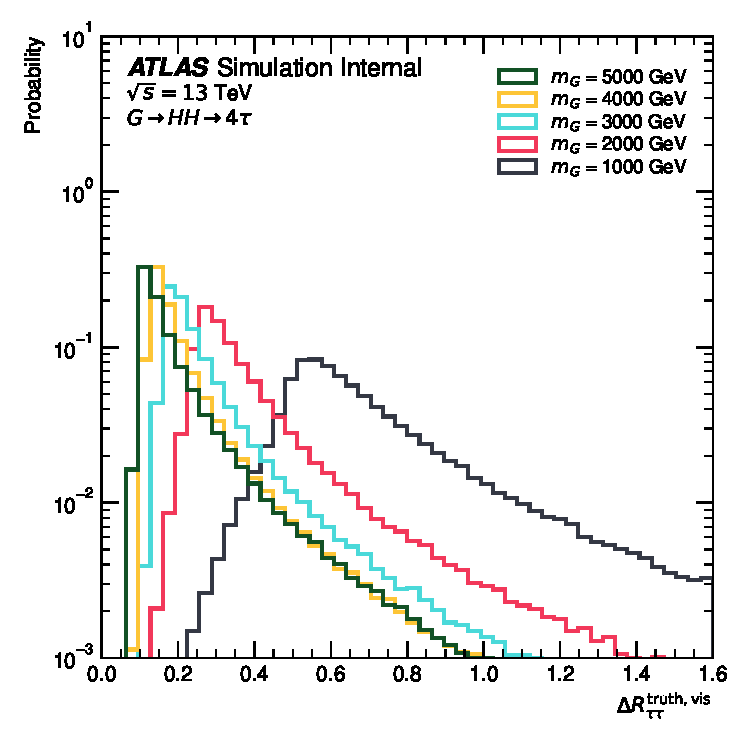
\includegraphics[width=0.50\textwidth]{plots_dev_fin/truth_dR_tt.pdf}
                \caption{The distributions of the $\dRtttruthvis$ between the truth 
                    level \tmth pair in the \GHHFourtau with hypothetical Graviton 
                    mass ranging from 1000 GeV to 5000 GeV. The distributions are normalised to unity.}
                \label{fig:murm:dr}
            \end{center}
        \end{figure}
        If the $\dRtttruthvis < 0.4$, it is likely that the muon will 
        be reconstructed inside the $\tauseed$ jet. 
        %However, for $\dRtttruthvis > 0.4$, the muon is not expected to overlap with the $\tauseed$ jet.

        For the purposes of this study, MC truth information is used to match truth-level $\tmth$ pairs with 
        their reconstructed counterparts. This facilitates focusing on only $\tauseed$ jets originating 
        from the boosted $\tmth$ pair and allows other $\tauseed$ jets associated with QCD jets to be neglected. 
        The MC truth-level visible $\tau$ decay products are required to satisfy the 
        requirements $p_T > 20\text{ \GeV}$ and $|\eta| < 2.5$, to ensure that the $\tauseed$ jets 
        are within the tracking acceptance of the ATLAS detector. 

        \begin{figure}[hbtp]
            \begin{center}
                \subfloat[]{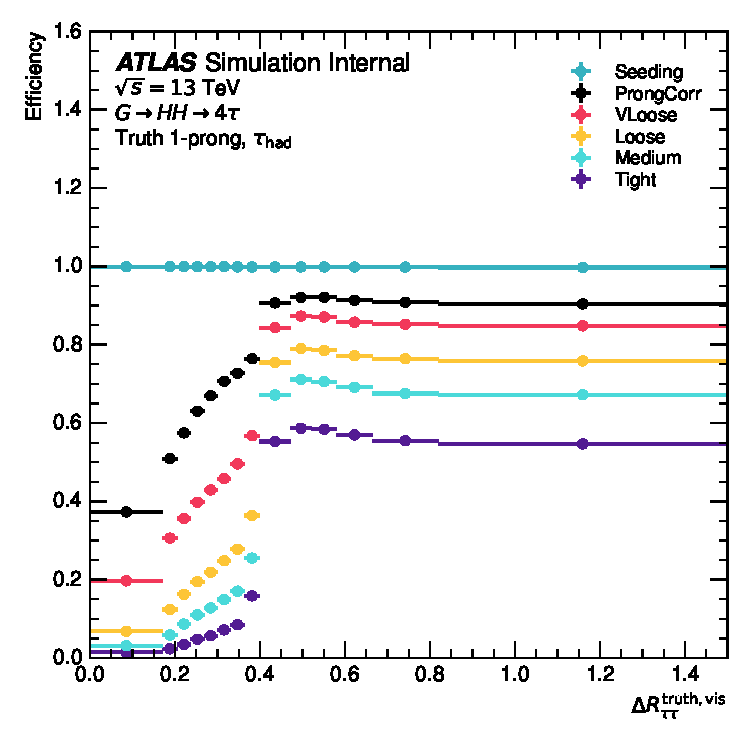
\includegraphics[width=0.5\textwidth]{plots_dev_fin/eff_nocut_dR_off_1p.pdf}\label{fig:murm:effi_off_1p}}
                \subfloat[]{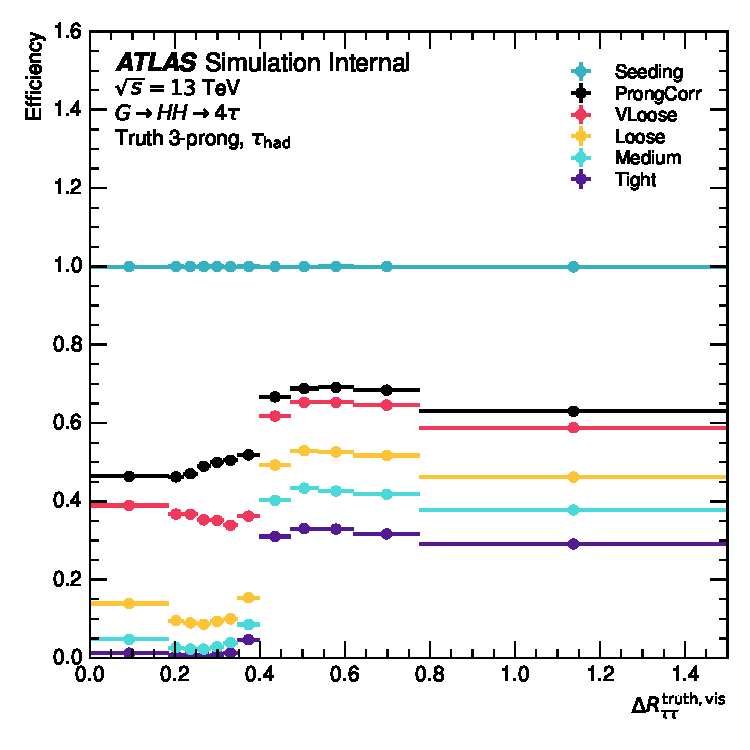
\includegraphics[width=0.5\textwidth]{plots_dev_fin/eff_nocut_dR_off_3p.pdf}\label{fig:murm:effi_off_3p}}
                \caption{The combined reconstruction and identification efficiencies of the standard ATLAS TauID for 
                    truth 1-prong~(\protect\subref{fig:murm:effi_off_1p}) and 3-prong~(\protect\subref{fig:murm:effi_off_3p}) $\tmth$ pairs 
                    in all working points as a function of $\dRtttruthvis$; the ``Seeding'' line 
                    (dark cyan) shows the efficiency of a $\tauseed$ jet that matches to a truth-level $\tmth$ pair being 
                    reconstructed; the ``ProngCorr'' line (black) shows the efficiency of a truth-level $\tauhad$ being 
                    reconstructed with the correct number of associated charged-particle tracks.
                }
                \label{fig:murm:effi_off}
            \end{center}
        \end{figure}

        The loss of performance of the standard TauID algorithm in the low $\dRtttruthvis$ 
        region is illustrated in Figure~\ref{fig:murm:effi_off}, which shows the combined reconstruction and identification efficiencies of 
        the standard ATLAS $\tauhad$ reconstruction algorithm and TauID algorithm as a function of $\dRtttruthvis$ for truth ``1-prong'' and ``3-prong'' 
        $\tmth$ pairs. Here the ``n-prong'' denotes the number of charged hadrons that originate from the $\tauhad$ decay. 
        The efficiency for a $\tauseed$ jet to be reconstructed from a truth-level $\tmth$ pair remains high for all 
        values of $\dRtttruthvis$. However, the efficiencies for all standard TauID working 
        points drop significantly in both ``1-prong'' and ``3-prong'' cases when $\dRtttruthvis < 0.4$. 
        The tighter the working point, the greater the fractional loss in efficiency due to the presence of the nearby
        muon. The performance of the standard TauID algorithm is set as a baseline in this study.

        The muon's nature as a minimum ionising particle, combined with the fact 
        that its reconstruction is independent of its isolation~\cite{MUON-2018-03}, 
        provides a motivation for excluding the inner detector track and calorimeter 
        clusters associated with any nearby muon from the the standard ATLAS $\tauhad$ reconstruction algorithm. 
        %Inclusion of their associated tracks and clusters could lead to contamination in the reconstruction of the $\tauseed$ jet. 
        By removing these contributions, the $\tauseed$ jet would better represent 
        only the hadronically decaying $\tau$, improving the accuracy of TauID.
        Specifically, the inner detector track and clusters associated with a reconstructed muon that 
        satisfies the ``Medium'' muon ID working point~\cite{MUON-2018-03} 
        is removed if the track or cluster is found within the reconstructed $\tauseed$ jet. 
        After the muon removal, the standard 
        hadronic tau reconstruction algorithm is re-run on the $\tauseed$ jet. In this way, the relevant ID variables for 
        the hadronically decaying $\tau$ can be calculated without the muon component.

    \subsection{Performance of the method} \label{sec:murm_perf}
        \begin{figure}[hbtp]
            \begin{center}
                \subfloat[]{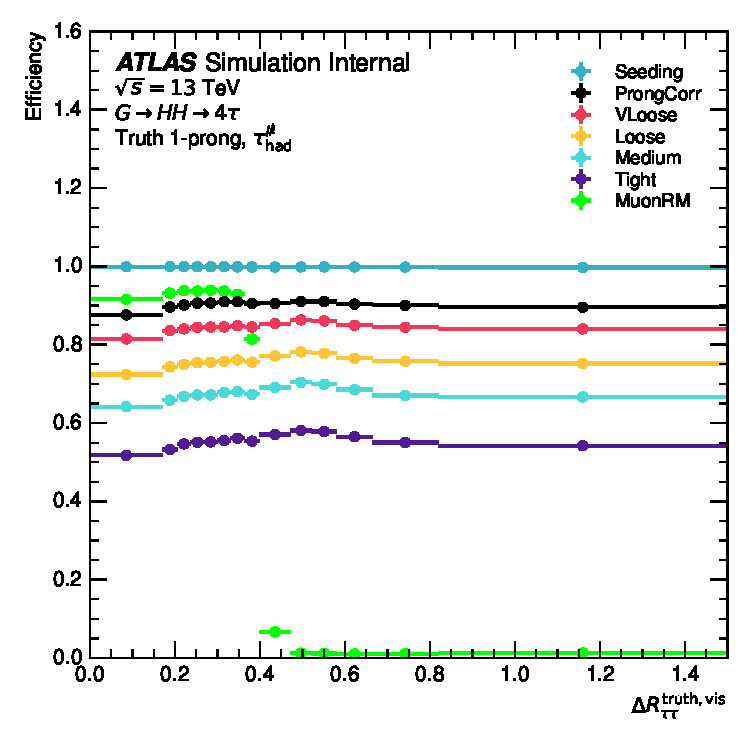
\includegraphics[width=0.5\textwidth]{plots_dev_fin/eff_nocut_dR_new_1p.pdf}\label{fig:murm:effi_new_1p}}
                \subfloat[]{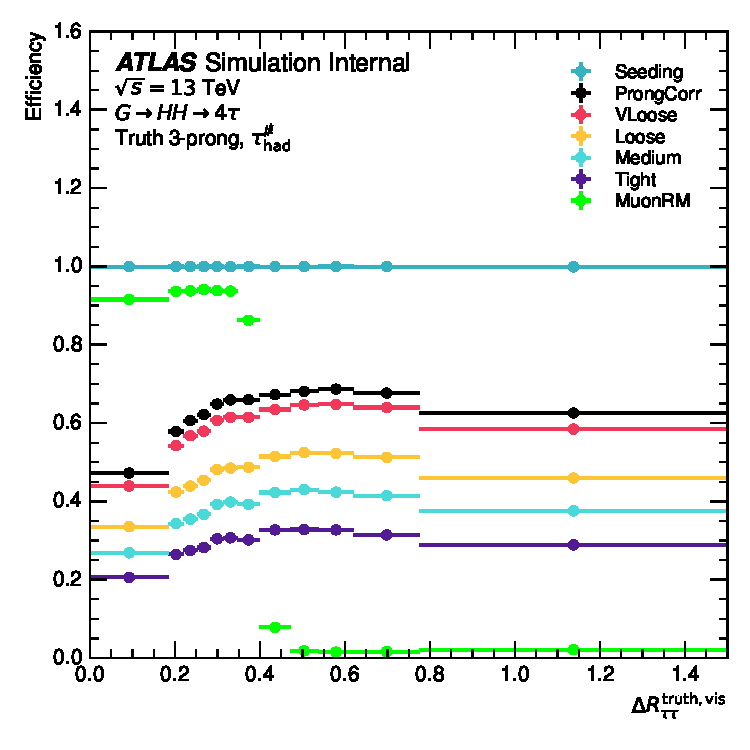
\includegraphics[width=0.5\textwidth]{plots_dev_fin/eff_nocut_dR_new_3p.pdf}\label{fig:murm:effi_new_3p}}
                \caption{The combined reconstruction and TauID efficiencies 
                    after the muon removal for truth 1-prong~(\protect\subref{fig:murm:effi_new_1p})
                    and 3-prong~(\protect\subref{fig:murm:effi_new_3p}) 
                    $\tmth$ pairs in all working points as a function of $\dRtttruthvis$. 
                    The extra ``MuonRM'' line (green) shows the efficiency of a muon 
                    being removed from the \tauseed. The slight abnormality in the ``MuonRM'' line 
                    between $0.35 < \dRtttruthvis < 0.45$ is due to limited detector 
                    resolution in the direction of the reconstructed $\tauhadvis$.
                }
                \label{fig:murm:effi_new}
            \end{center}
        \end{figure}
        Figure~\ref{fig:murm:effi_new} shows the combined reconstruction and identification efficiencies after muon removal as a function of 
        $\dRtttruthvis$ for truth 1-prong and 3-prong $\tmth$ pairs in all working points. 
        The reconstruction and identification efficiencies after muon removal show a considerable improvement compared to those shown 
        in Figure~\ref{fig:murm:effi_off}. The signal efficiency is recovered almost completely in every working point 
        for both 1-prong and 3-prong $\tauhad$. For 3-prong cases, the efficiency of TauID is limited by the 
        accurate reconstruction of the correct number of tracks associated with the highly boosted 
        $\tauhad$ (referred to as ``ProngCorr''). 
        % The performance metrics for the identification of 3-prong 
        % $\tauhad$ without incorporating the ``ProngCorr'' criterion are presented in the Appendix. 
        % A full recovery of the signal efficiency for the identification of 3-prong $\tauhad$.


        Roughly 95\% of the $\tauseed$ jets have a muon removed in the region where $\dRtttruthvis < 0.4$. 
        This can be expected given the 97\% efficiency of the ``Medium'' muon ID working point, 
        with a dip below 90\% in the region $\absetatruthvis < 0.1$. This is illustrated in 
        Figure~\ref{fig:murm:etaRM}, which shows the signal efficiencies of the TauID working points after muon removal as a 
        function of the $\absetatruthvis$ for truth 1-prong and 3-prong $\tauseed$ jets with 
        $\dRtttruthvis < 0.4$. 
        % The dip in efficiency for $\absetatruthvis < 0.1$ is caused by
        % the muon identification inefficiency for central muons.

        \begin{figure}[hbtp]
            \begin{center}
                \subfloat[]{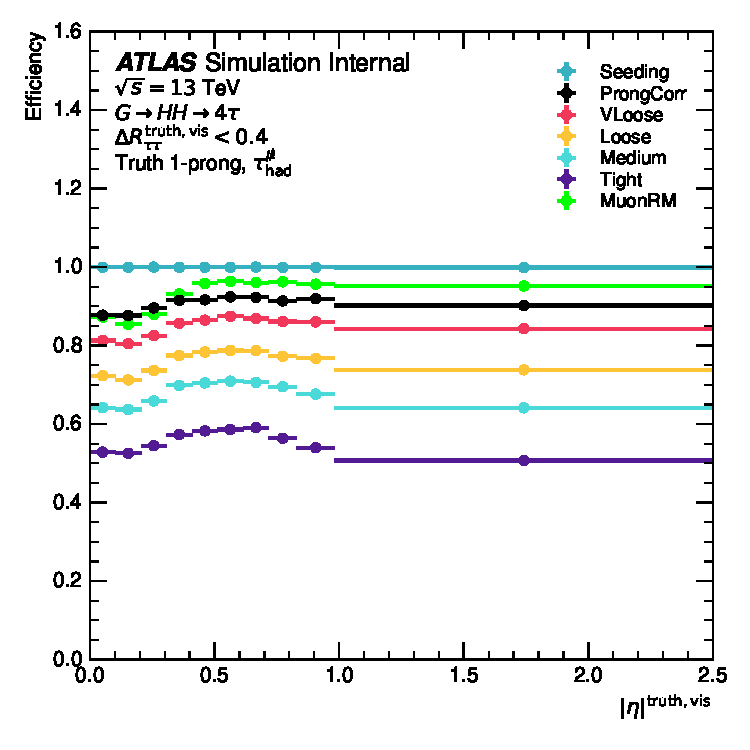
\includegraphics[width=0.50\textwidth]{plots_dev_fin/eff_dR04_eta_new_1p.pdf}\label{fig:murm:etaRM_1p}}
                \subfloat[]{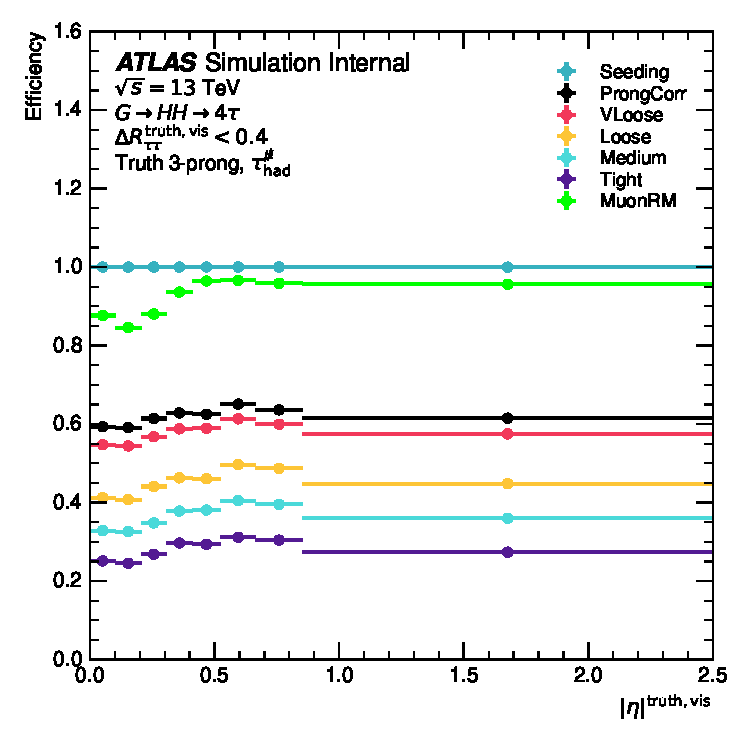
\includegraphics[width=0.50\textwidth]{plots_dev_fin/eff_dR04_eta_new_3p.pdf}\label{fig:murm:etaRM_3p}}
                \caption{The signal efficiencies of the TauID working points as a function of the truth absolute pseudorapidity 
                for truth 1-prong~(\protect\subref{fig:murm:etaRM_1p}) and 3-prong~(\protect\subref{fig:murm:etaRM_3p}) $\tauseed$ jets
                with $\dRtttruthvis < 0.4$. The seeding efficiencies and the ratio of the 
                $\tauseed$ jets with a muon removed are also shown.}
                \label{fig:murm:etaRM}
            \end{center}
        \end{figure}

        The signal identification efficiencies in all working points of the standard ATLAS TauID are tuned to show minimum 
        dependency on the $\pttautruthvis$ and pile-up~\cite{ATL-PHYS-PUB-2019-033}. The stability 
        of the TauID working point efficiencies after muon removal against these variables is shown in Figure~\ref{fig:murm:stability}. 
        To focus on the objects of interest, only truth $\tmth$ pairs with the $\Delta R$ between the reconstructed muon and $\tauhad$, $\dRttreco < 0.4$ 
        are included in the plots. For comparison, the TauID working point efficiencies as a function of the same variables 
        for $\tauseed$ objects in which muon removal is not required ($\dRtttruthvis > 0.45$) 
        are shown in Figure~\ref{fig:murm:45drstability}. Similar behaviour is observed in figures~\ref{fig:murm:stability} and~\ref{fig:murm:45drstability}. 
        The improved performance and good stabilities across different working points demonstrate that, after muon removal, 
        the TauID RNN sees the signal $\tauseed$ jet as if it were a $\tauhad$ that is free from interference of surrounding particles (isolated $\tauhad$).

        \begin{figure}[hbtp]
            \begin{center}
                \subfloat[]{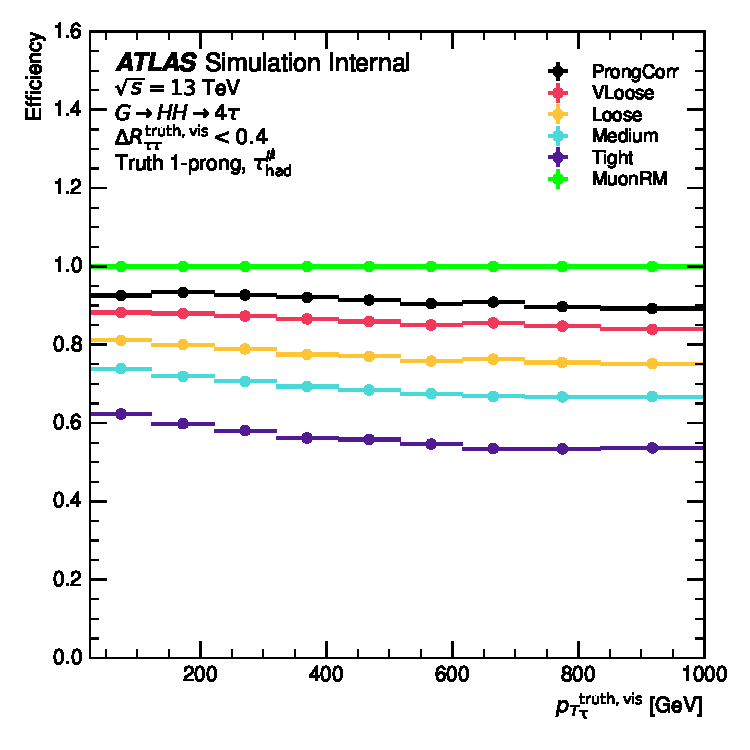
\includegraphics[width=0.50\textwidth]{plots_dev_fin/eff_dR04_murm_pt_new_1p.pdf} \label{fig:murm:ptDR04_1p}}  
                \subfloat[]{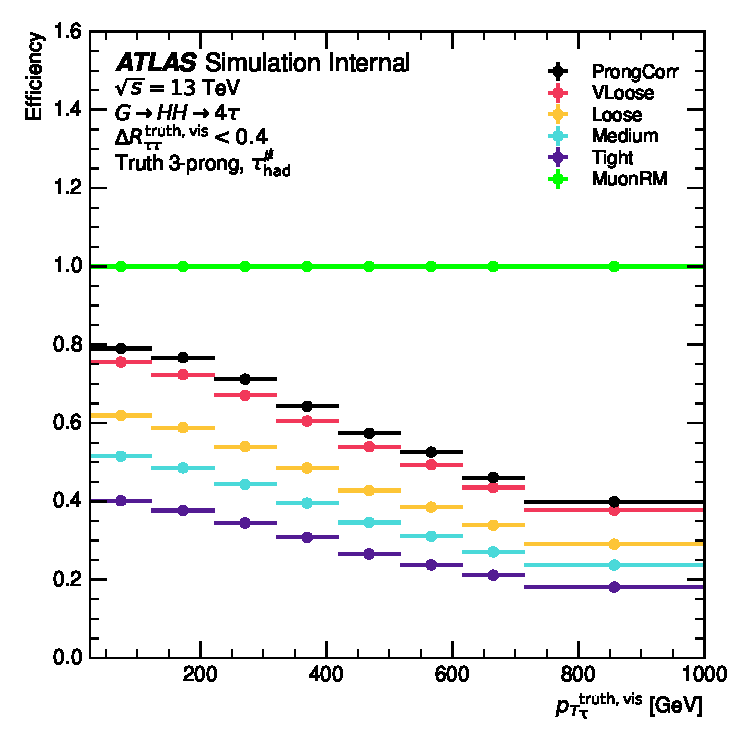
\includegraphics[width=0.50\textwidth]{plots_dev_fin/eff_dR04_murm_pt_new_3p.pdf} \label{fig:murm:ptDR04_3p}}  
                \vspace{-0.45cm} % Adjust the negative space here to bring rows closer
                \\
                % \subfloat[]{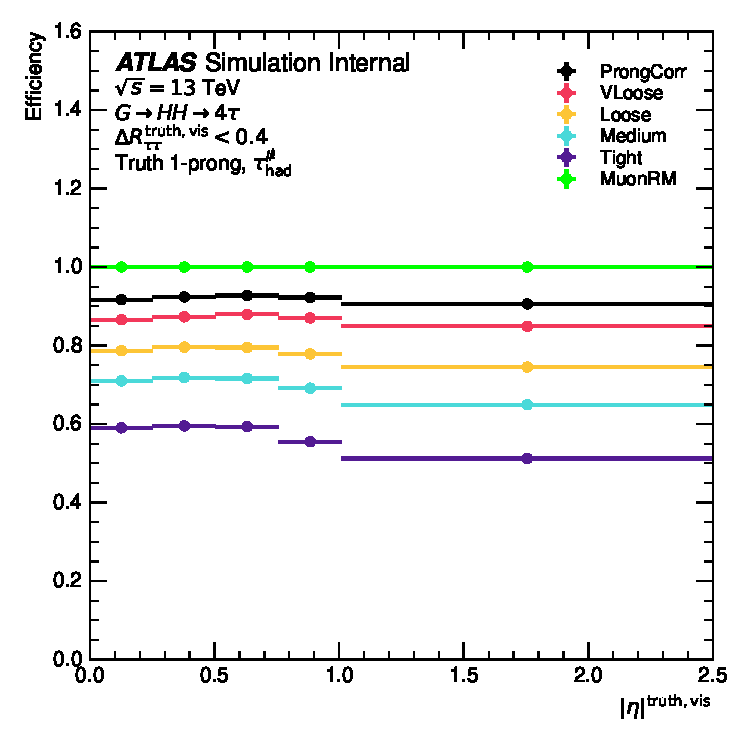
\includegraphics[width=0.50\textwidth]{plots_dev_fin/eff_dR04_murm_eta_new_1p.pdf}\label{fig:murm:etaDR04_1p}}
                % \subfloat[]{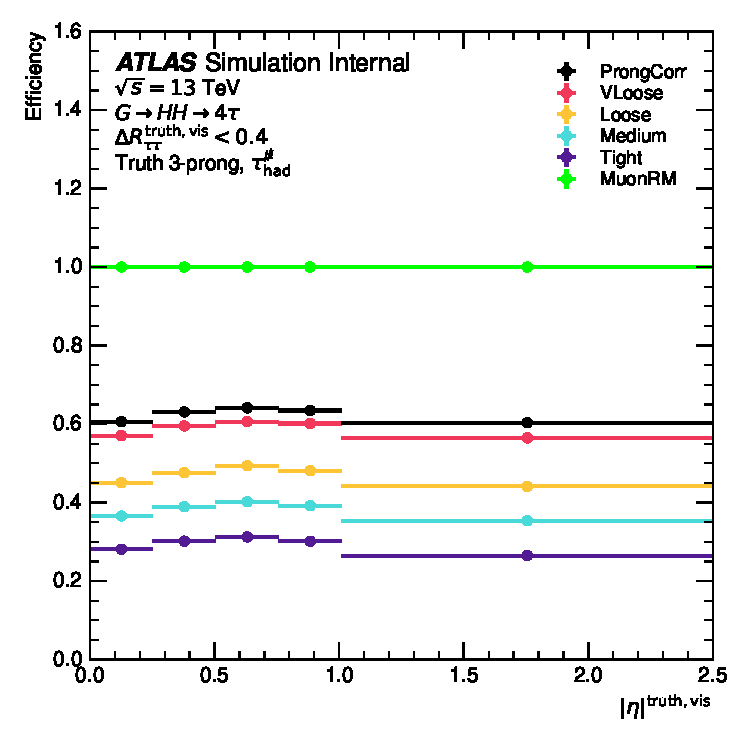
\includegraphics[width=0.50\textwidth]{plots_dev_fin/eff_dR04_murm_eta_new_3p.pdf}\label{fig:murm:etaDR04_3p}}
                % \vspace{-0.45cm} % Adjust the negative space here to bring rows closer
                % \\
                \subfloat[]{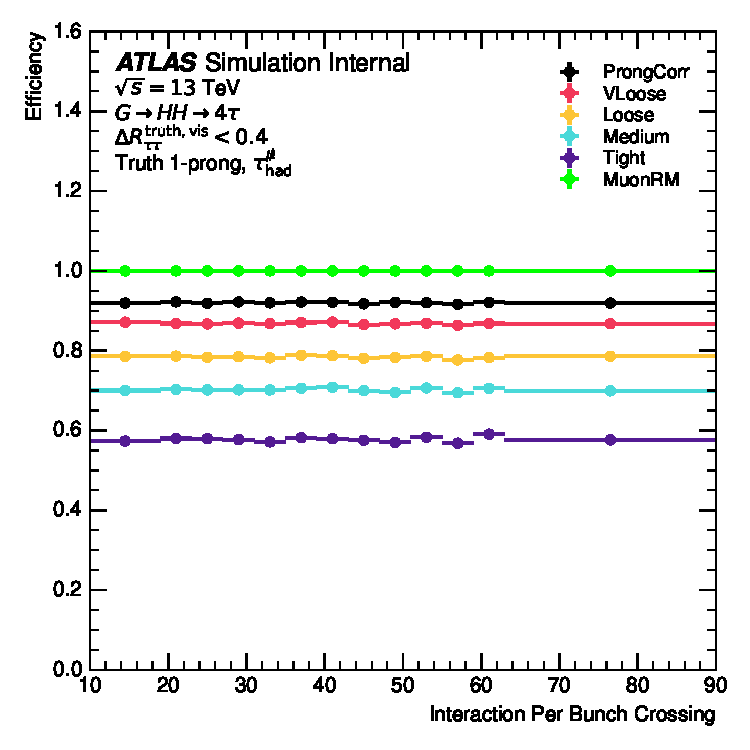
\includegraphics[width=0.50\textwidth]{plots_dev_fin/eff_dR04_murm_mu_new_1p.pdf} \label{fig:murm:muDR04_1p}}  
                \subfloat[]{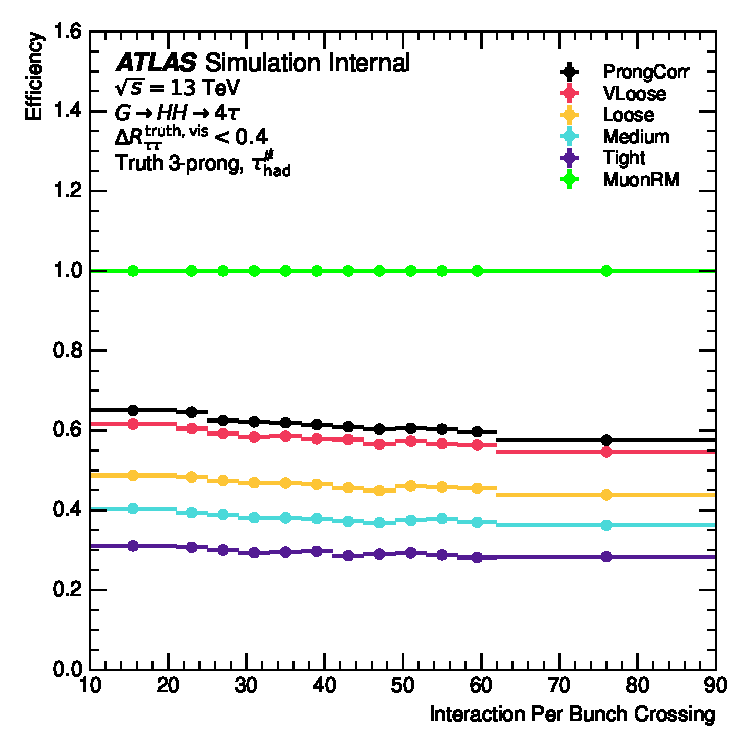
\includegraphics[width=0.50\textwidth]{plots_dev_fin/eff_dR04_murm_mu_new_3p.pdf} \label{fig:murm:muDR04_3p}}  
                \caption{The stability of the signal efficiencies of the TauID working points against 
                    the truth transverse momentum~(\protect\subref{fig:murm:ptDR04_1p})~(\protect\subref{fig:murm:ptDR04_3p}), 
                    % absolute pseudorapidity~(\protect\subref{fig:murm:etaDR04_1p})~(\protect\subref{fig:murm:etaDR04_3p}), 
                    and pile-up~(\protect\subref{fig:murm:muDR04_1p})~(\protect\subref{fig:murm:muDR04_3p}) for truth 
                    1-prong and 3-prong $\tauseed$ with reconstructed $\dRttreco < 0.4$.
                    The ``Seeding'' lines indicate the efficiency 
                    of a truth-level $\tauhad$ being reconstructed as $\tauseed$. The ``MuonRM'' lines show the efficiency of 
                    a muon being removed inside the $\tauseed$.
                }
                \label{fig:murm:stability}
            \end{center}
        \end{figure}

        \begin{figure}[hbtp]
            \begin{center}
                \subfloat[]{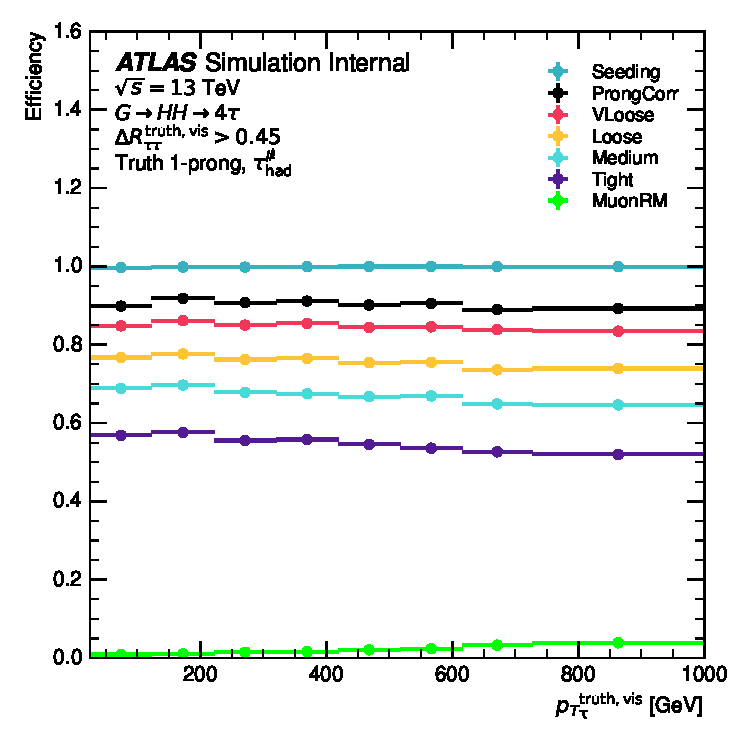
\includegraphics[width=0.50\textwidth]{plots_dev_fin/eff_04dR_pt_new_1p.pdf}  \label{fig:murm:pt45dr_1p}}
                \subfloat[]{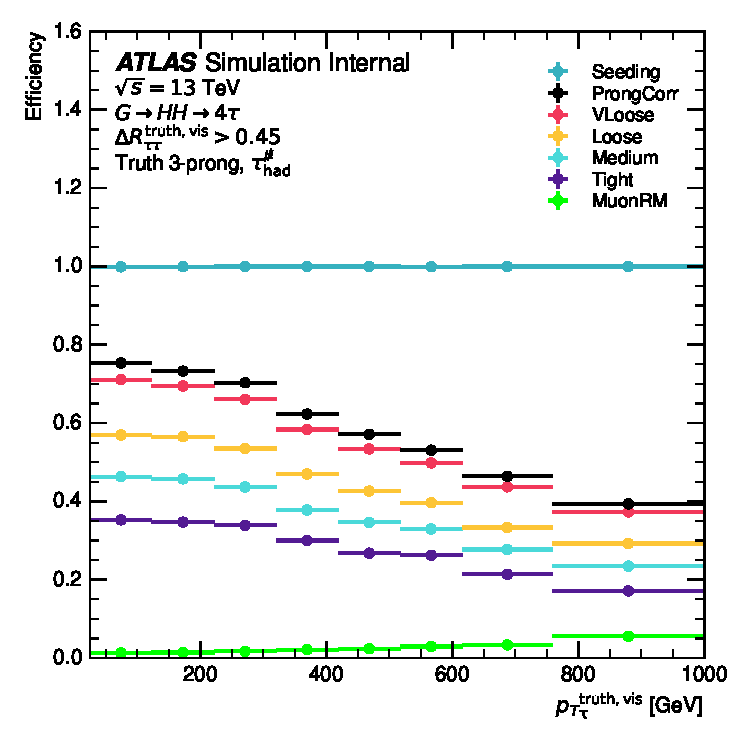
\includegraphics[width=0.50\textwidth]{plots_dev_fin/eff_04dR_pt_new_3p.pdf}  \label{fig:murm:pt45dr_3p}}
                \vspace{-0.45cm} % Adjust the negative space here to bring rows closer
                \\
                % \subfloat[]{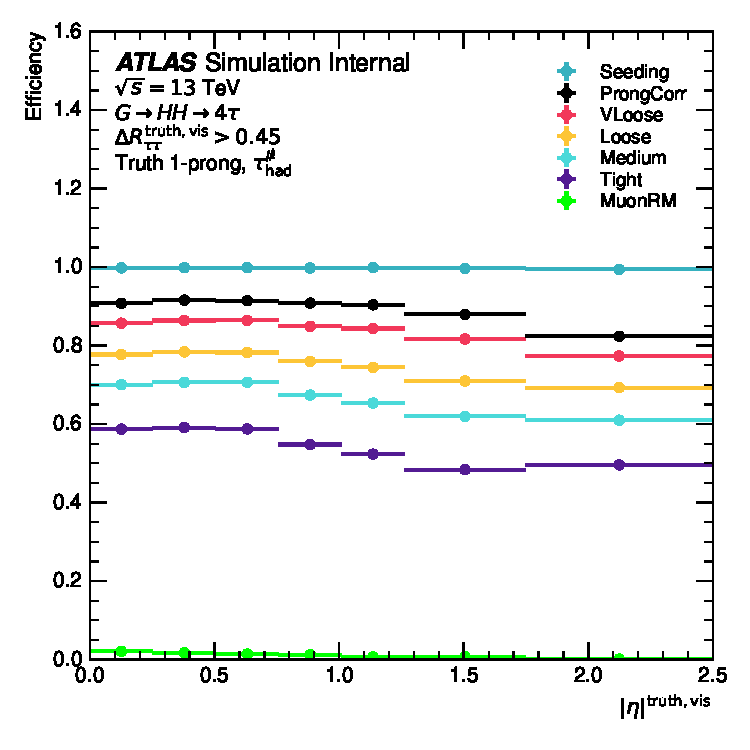
\includegraphics[width=0.50\textwidth]{plots_dev_fin/eff_04dR_eta_new_1p.pdf} \label{fig:murm:eta45dr_1p}}
                % \subfloat[]{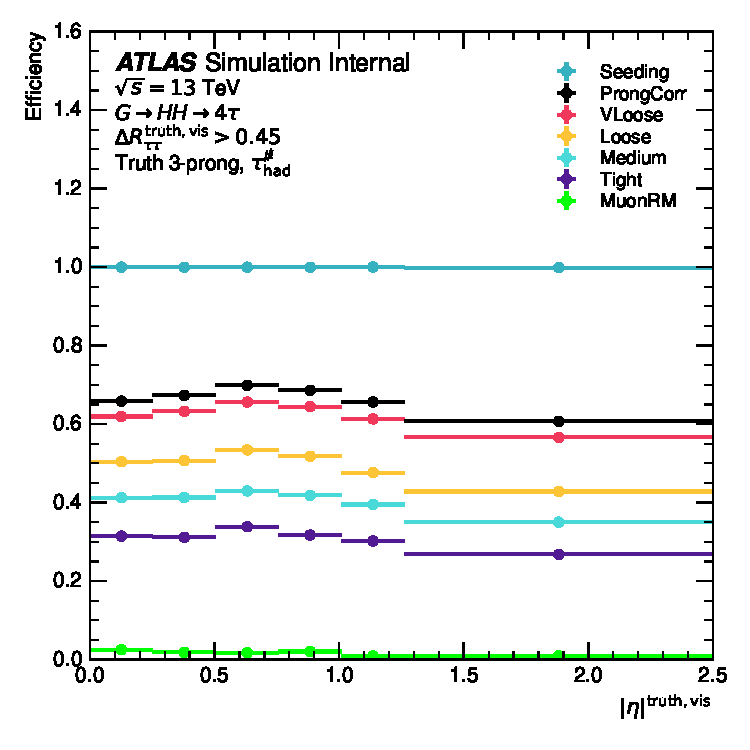
\includegraphics[width=0.50\textwidth]{plots_dev_fin/eff_04dR_eta_new_3p.pdf} \label{fig:murm:eta45dr_3p}}
                % \vspace{-0.45cm} % Adjust the negative space here to bring rows closer
                % \\
                \subfloat[]{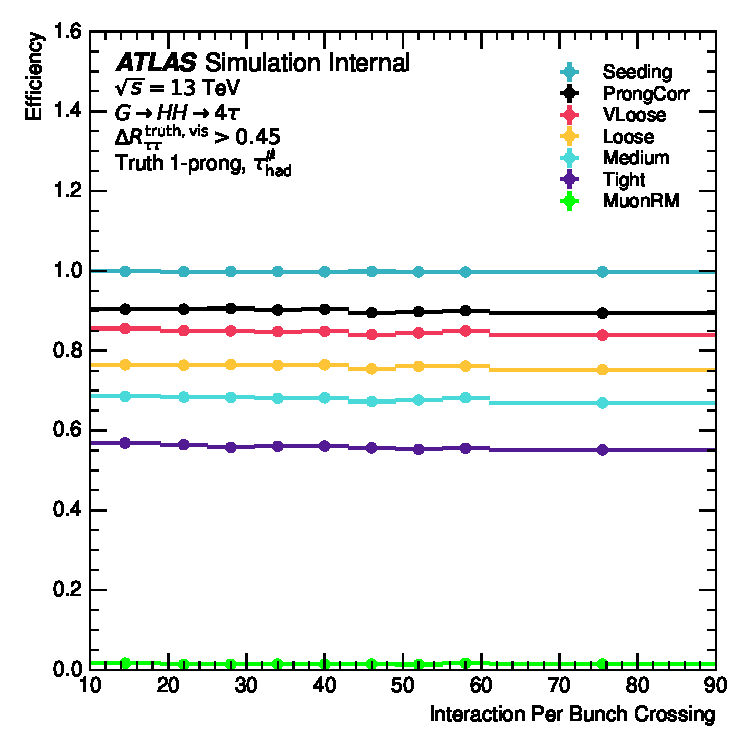
\includegraphics[width=0.50\textwidth]{plots_dev_fin/eff_04dR_mu_new_1p.pdf}  \label{fig:murm:mu45dr_1p}}
                \subfloat[]{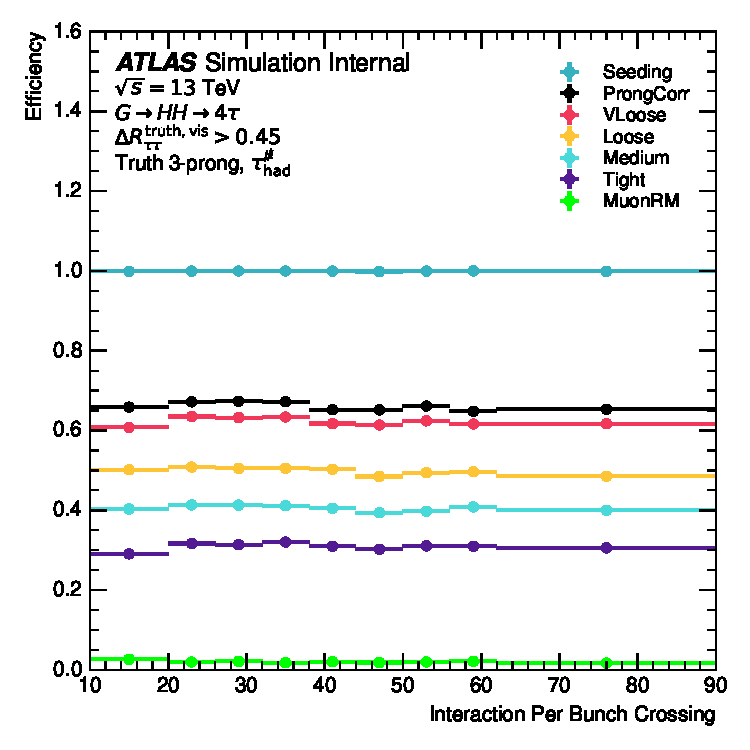
\includegraphics[width=0.50\textwidth]{plots_dev_fin/eff_04dR_mu_new_3p.pdf}  \label{fig:murm:mu45dr_3p}}
                \caption{The stability of the signal efficiencies of the TauID working points against 
                    the truth transverse momentum~(\protect\subref{fig:murm:pt45dr_1p})~(\protect\subref{fig:murm:pt45dr_3p}), 
                    % absolute pseudorapidity~(\protect\subref{fig:murm:eta45dr_1p})~(\protect\subref{fig:murm:eta45dr_3p}), 
                    and pile-up~(\protect\subref{fig:murm:mu45dr_1p})~(\protect\subref{fig:murm:mu45dr_3p}) for 
                    the truth 1-prong and 3-prong $\tauseed$ jets with $\dRtttruthvis > 0.45$. 
                    In this region, the muon removal should not affect the results. The ``Seeding'' lines indicate the efficiency 
                    of a truth-level $\tauhad$ being reconstructed as $\tauseed$. The ``MuonRM'' lines show the efficiency of 
                    a muon being removed inside the $\tauseed$.}
                \label{fig:murm:45drstability}
            \end{center}
        \end{figure}

        After the removal of the overlapping muon, the precision with which the four-momentum of the $\tauseed$ jet is reconstructed 
        improves significantly. Figure~\ref{fig:murm:sp_resolutions} shows the distributions of 
        the difference between the truth-level and reconstructed variable (residuals) 
        in $\eta$ and $\phi$ before and after muon removal. Compared to the performance before muon removal, the root mean square (RMS)
        widths of the $\eta$ residuals that correspond to the 68\% percentile (core resolution) 
        improves by a factor of 15 for 1-prong $\tauhad$, and by a factor of 20 for 3-prong $\tauhad$. 
        The core resolution in $\phi$ improves also by a factor of 15 times for 1-prong $\tauhad$ and by a factor of 20 for 3-prong $\tauhad$. 
        The distributions of the $\tauhadvis$ transverse energy ($E_\mathrm{T}$) residuals and the relative core (68\%) and 
        tail (95\%) $E_\mathrm{T}$ resolutions as functions of $\tauhadvis$ $E_\mathrm{T}^\mathrm{truth}$ are shown in 
        Figure~\ref{fig:murm:e_resolutions}. These results align nicely with those reported for isolated $\tauhad$ in ref.~\cite{PERF-2014-06}, 
        demonstrating further the effectiveness of the muon-removal technique.

        \begin{figure}[hbtp]
            \begin{center}
                \subfloat[]{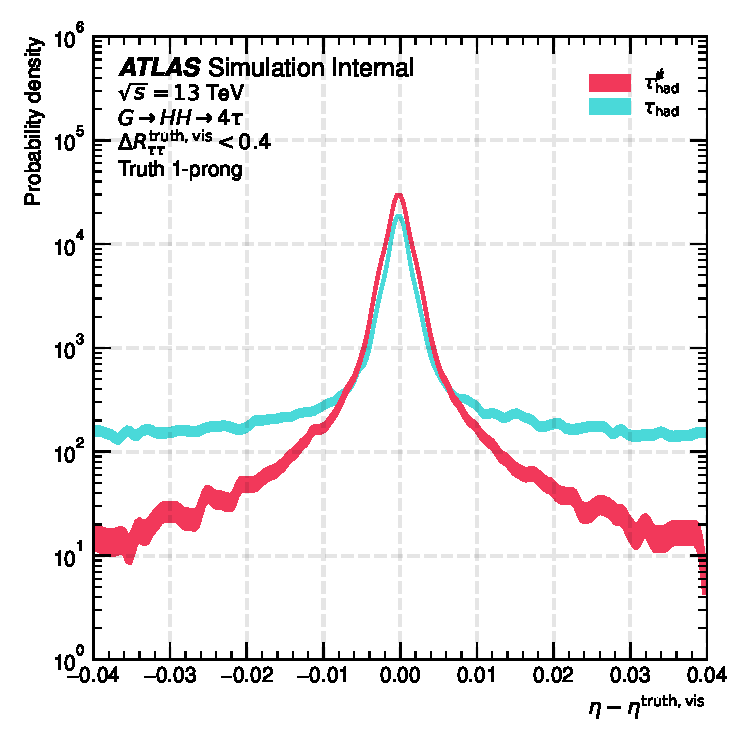
\includegraphics[width=0.5\textwidth]{plots_dev_fin/reso_eta_diff_1p.pdf} \label{fig:murm:reso_eta_1p}}
                \subfloat[]{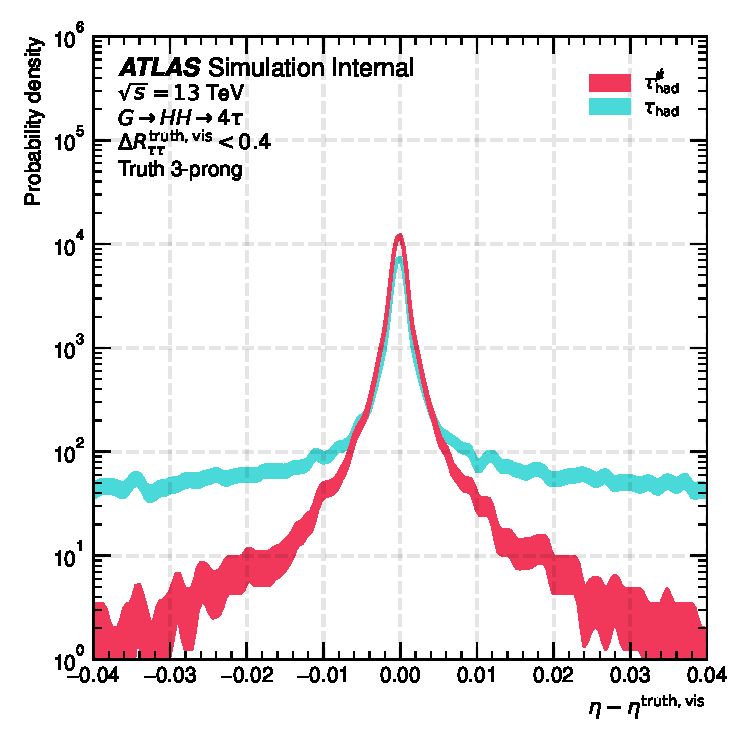
\includegraphics[width=0.5\textwidth]{plots_dev_fin/reso_eta_diff_3p.pdf} \label{fig:murm:reso_eta_3p}}
                \\
                \subfloat[]{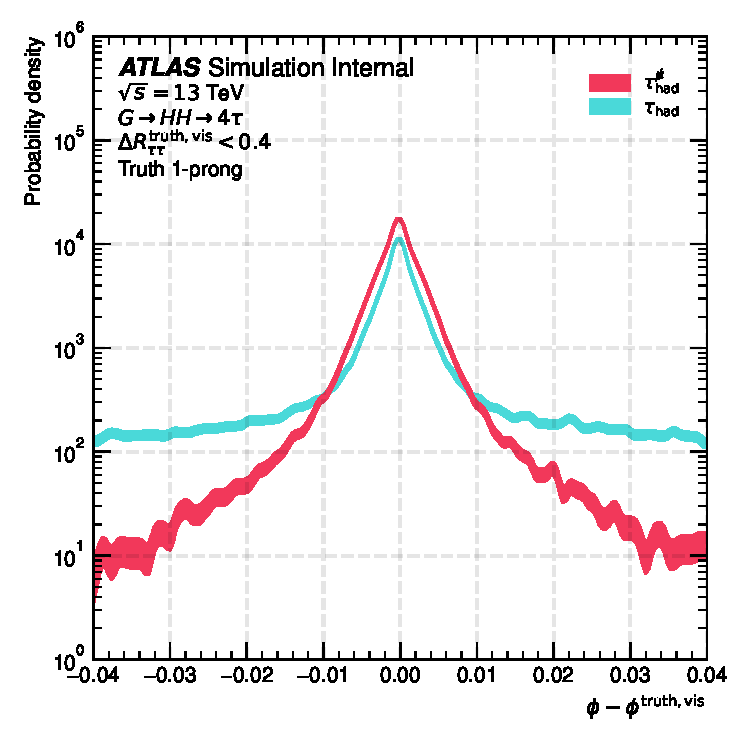
\includegraphics[width=0.5\textwidth]{plots_dev_fin/reso_phi_diff_1p.pdf} \label{fig:murm:reso_phi_1p}}
                \subfloat[]{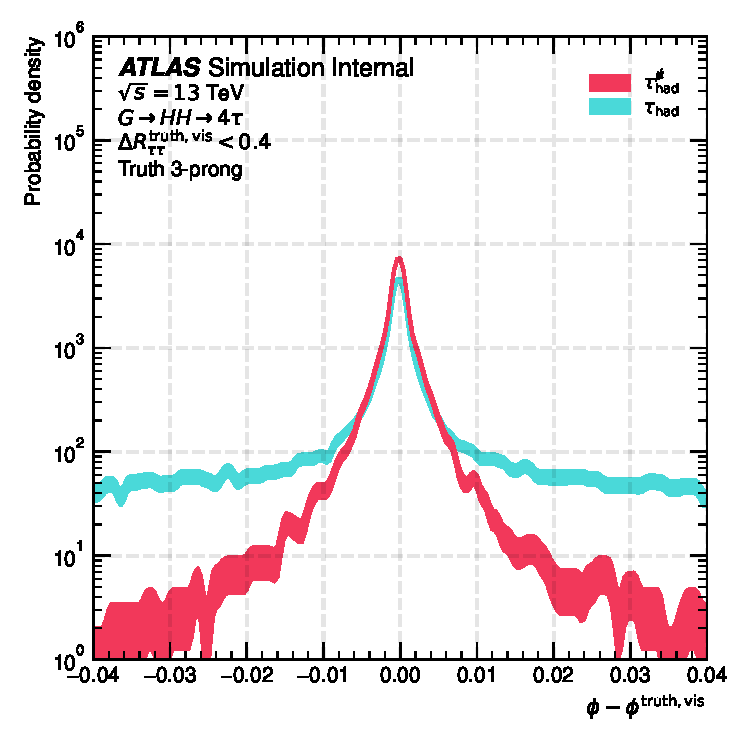
\includegraphics[width=0.5\textwidth]{plots_dev_fin/reso_phi_diff_3p.pdf} \label{fig:murm:reso_phi_3p}}
                \caption{The distributions of the calibrated residuals 
                    $\eta$~(\protect\subref{fig:murm:reso_eta_1p})~(\protect\subref{fig:murm:reso_eta_3p}) and 
                    $\phi$~(\protect\subref{fig:murm:reso_phi_1p})~(\protect\subref{fig:murm:reso_phi_3p}) 
                    before (blue) and after (red) muon removal. The left panel shows the 1-prong case; the right 
                    panel shows the 3-prong case.}
                \label{fig:murm:sp_resolutions}
            \end{center}
        \end{figure}
        \begin{figure}[hbtp]
            \begin{center}
                \subfloat[]{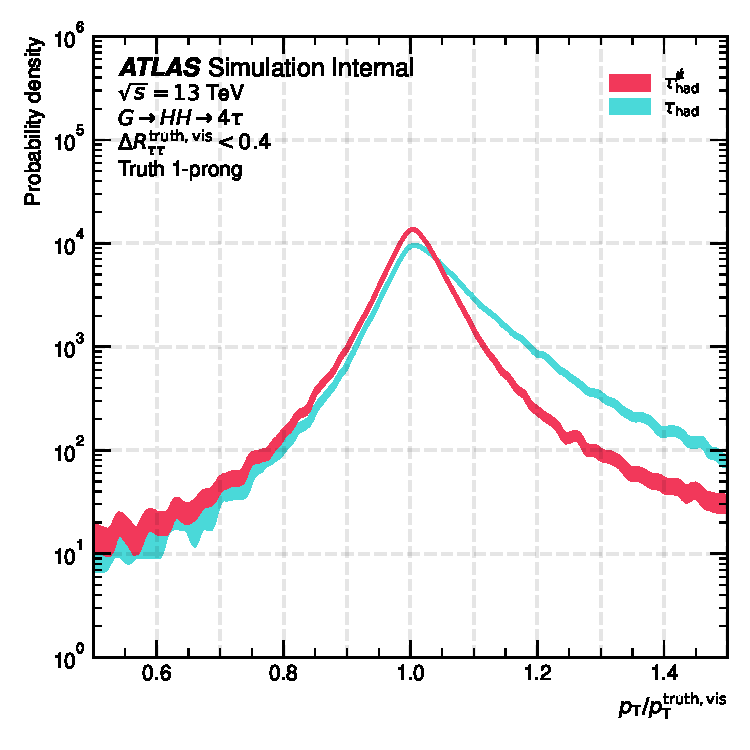
\includegraphics[width=0.5\textwidth]{plots_dev_fin/reso_pt_diff_1p.pdf}\label{fig:murm:reso_pt_1p}}
                \subfloat[]{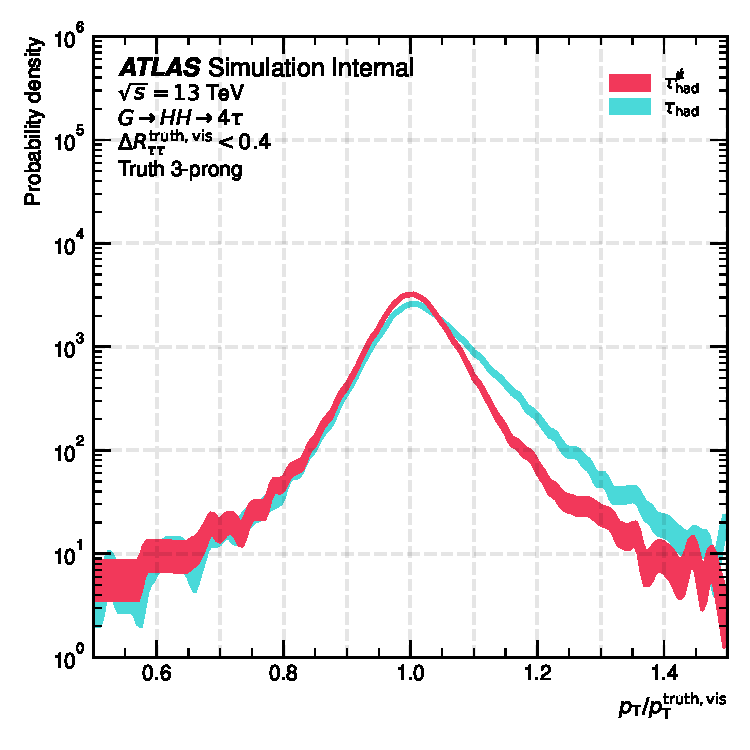
\includegraphics[width=0.5\textwidth]{plots_dev_fin/reso_pt_diff_3p.pdf}\label{fig:murm:reso_pt_3p}}
                \\
                \subfloat[]{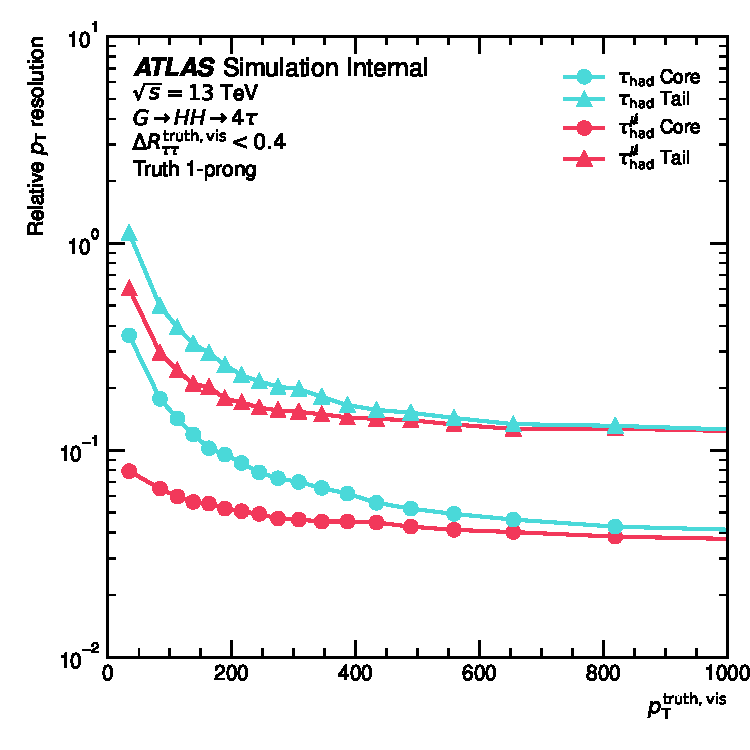
\includegraphics[width=0.5\textwidth]{plots_dev_fin/reso_rela_pt_1p.pdf}\label{fig:murm:reso_rel_pt_1p}}
                \subfloat[]{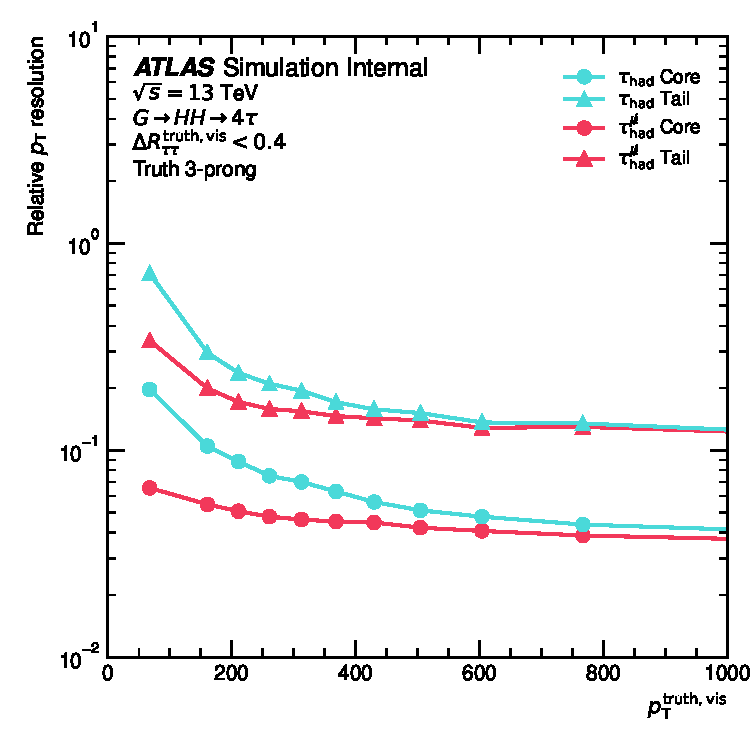
\includegraphics[width=0.5\textwidth]{plots_dev_fin/reso_rela_pt_3p.pdf}\label{fig:murm:reso_rel_pt_3p}}
                \caption{(\protect\subref{fig:murm:reso_pt_1p})~(\protect\subref{fig:murm:reso_pt_3p}): the distributions of the calibrated transverse energy 
                residuals for $\tauhadvis$ with (red) and without (blue) muon removal. 
                (\protect\subref{fig:murm:reso_rel_pt_1p})~(\protect\subref{fig:murm:reso_rel_pt_3p}): the relative core (68\%) and tail (95\%) 
                $\tauhadvis$ $E_\mathrm{T}$ resolutions as functions of $\tauhadvis$ $E_\mathrm{T}^\mathrm{truth}$. The left 
                plots show the 1-prong case and the right plots show the 3-prong case.}
                \label{fig:murm:e_resolutions}
            \end{center}
        \end{figure}

        Having demonstrated that the reconstruction and identification efficiencies are significantly improved by the $\tauhadmurm$ method, 
        the background rejection power is now illustrated. The production of \ttbar pairs is considered as a source of 
        high $\pt$ heavy-flavour jets, which represents an example background to the $\tauhadmurm$ signal.
        The background rejection ratios at the medium TauID working point, which are defined as the 
        inverted ratios of a mis-reconstructed $\tauseed$ jet being classified as a genuine $\tauhad$ are shown in Figure~\ref{fig:murm:rej},
        as functions of the reconstructed $\tauhad~\pt$, $\tauhad~|\eta|$ and pile-up. For the background rejection plots, and the following 
        receiver operating characteristic (ROC) plots, event-selections are mostly based on the reconstructed properties instead of the truth-level 
        information. A $\tauseed$ jet reconstructed in the background sample is required to have 
        $20\text{ \GeV}<\pt<300\text{ \GeV}$, 
        $|\eta|<2.5$, 
        and to not be truth-matched to a $\tauhad$ lepton from the bottom or top quarks semi-leptonic decay. 
        In addition, a reconstructed muon is required to be found inside the $\tauseed$ jet. 
        The $\tauhad$ candidates in which no muon is present are not considered in Figure~\ref{fig:murm:rej}, as identical 
        TauID results would be expected for these cases.

        \begin{figure}[hbtp]
            \begin{center}
                \subfloat[]{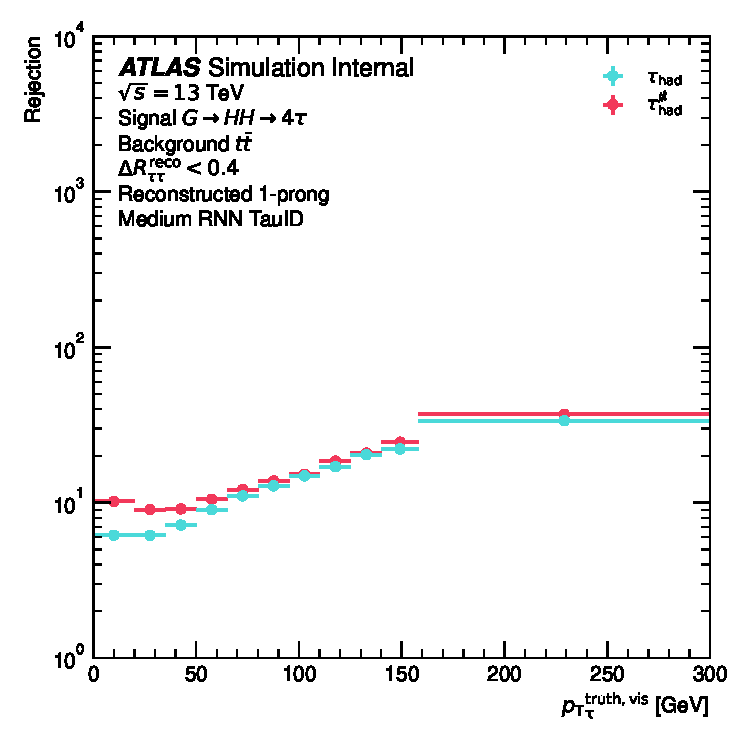
\includegraphics[width=0.5\textwidth]{plots_dev_fin/rej_pt_1p.pdf}  \label{fig:murm:rej_pt_1p}}
                \subfloat[]{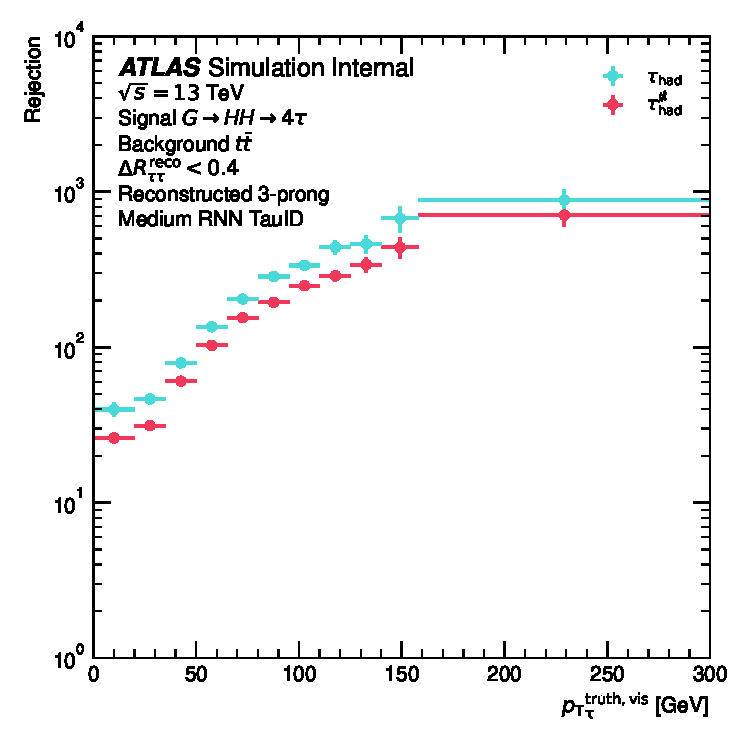
\includegraphics[width=0.5\textwidth]{plots_dev_fin/rej_pt_3p.pdf}  \label{fig:murm:rej_pt_3p}}
                \vspace{-0.45cm} % Adjust the negative space here to bring rows closer
                \\
                % \subfloat[]{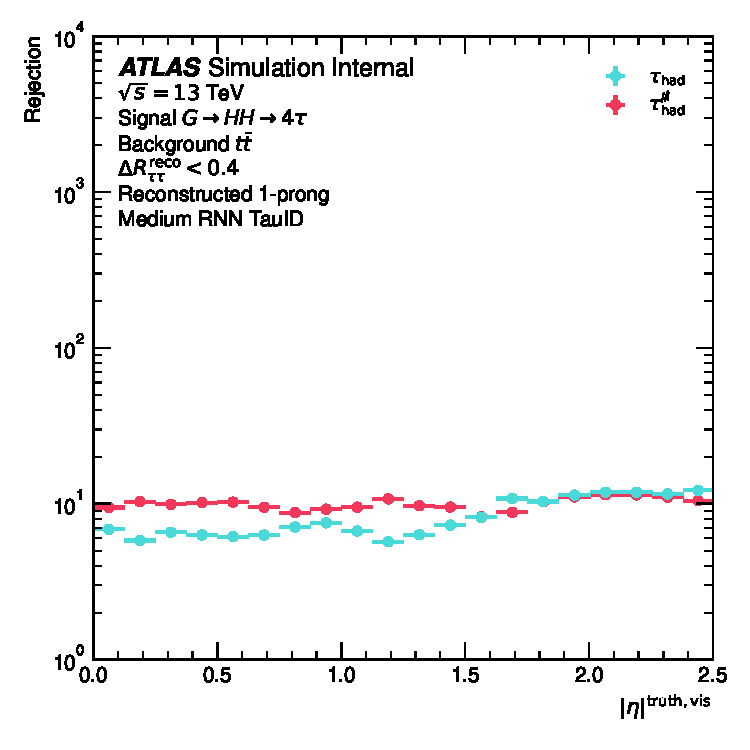
\includegraphics[width=0.5\textwidth]{plots_dev_fin/rej_eta_1p.pdf} \label{fig:murm:rej_eta_1p}}
                % \subfloat[]{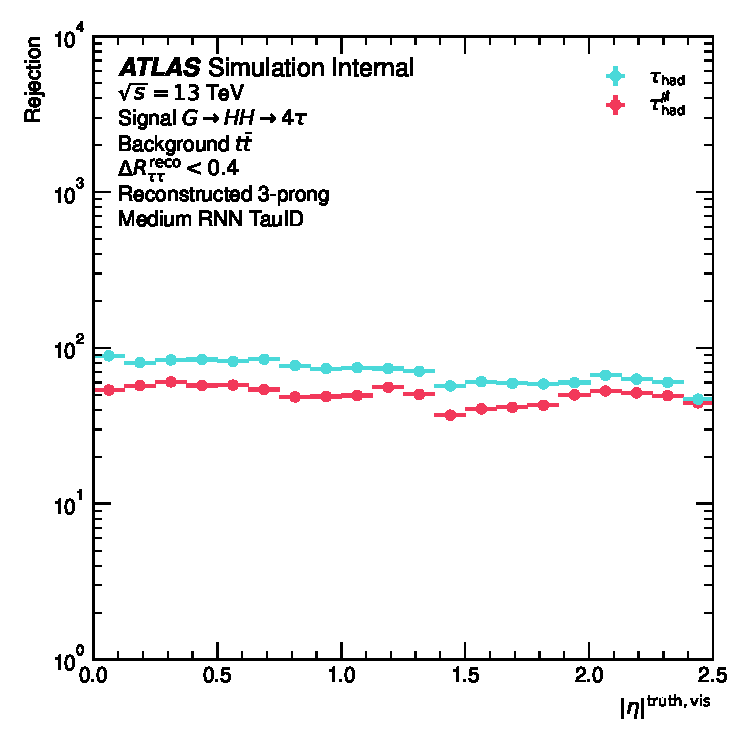
\includegraphics[width=0.5\textwidth]{plots_dev_fin/rej_eta_3p.pdf} \label{fig:murm:rej_eta_3p}}
                % \vspace{-0.45cm} % Adjust the negative space here to bring rows closer
                % \\
                \subfloat[]{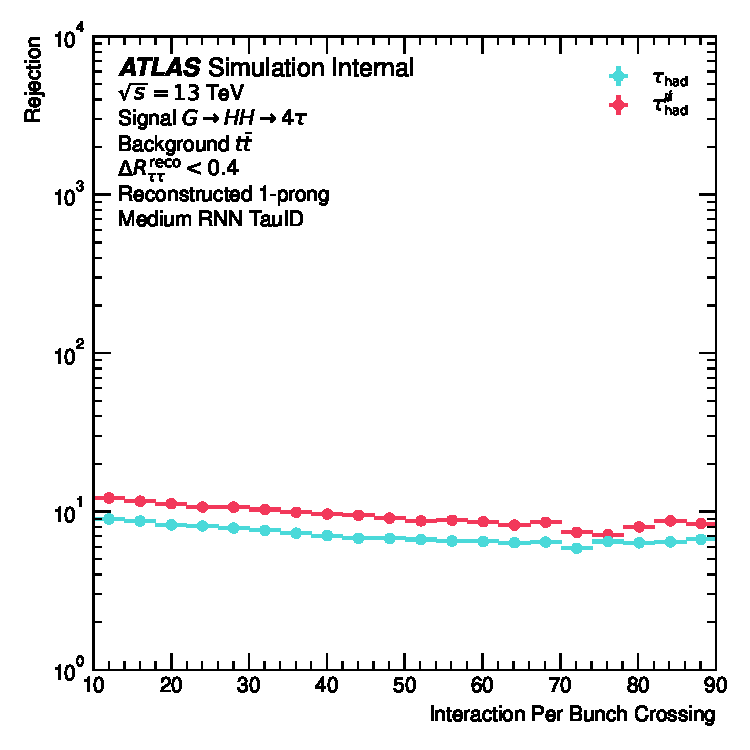
\includegraphics[width=0.5\textwidth]{plots_dev_fin/rej_mu_1p.pdf}  \label{fig:murm:rej_mu_1p}}
                \subfloat[]{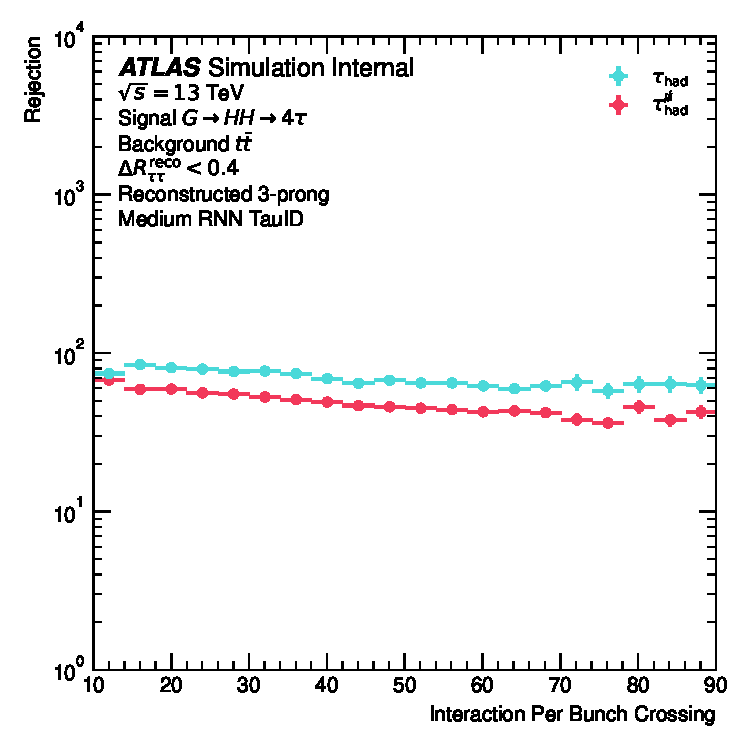
\includegraphics[width=0.5\textwidth]{plots_dev_fin/rej_mu_3p.pdf}  \label{fig:murm:rej_mu_3p}}
                \caption{The signal rejection ratios for $\tauseed$ jets reconstructed from jets originating from 
                semi-muonic bottom decays in \ttbar events at medium TauID working point, as functions of the 
                reconstructed \pt~(\protect\subref{fig:murm:rej_pt_1p})~(\protect\subref{fig:murm:rej_pt_3p}),
                % $|\eta|$~(\protect\subref{fig:murm:rej_eta_1p})~(\protect\subref{fig:murm:rej_eta_3p}), and 
                and pile-up~(\protect\subref{fig:murm:rej_mu_1p})~(\protect\subref{fig:murm:rej_mu_3p}). 
                The left panel shows the reconstructed 1-prong case, the right panel shows the 3-prong case.}
                \label{fig:murm:rej}
            \end{center}
        \end{figure}

        The background rejection power decreases slightly in the 3-prong case. 
        After the removal of the muon within the $\tau_\mathrm{seed}$ in the case of background events, 
        the TauID algorithm finds it more challenging to reject a semi-leptonic heavy-flavour jet.
        The 1-prong background rejection power increases slightly in 
        the low \pt region after removal of the muon due to two competing phenomena. 
        The muon being removed is often the only charged track found inside the $\tauseed$ jet. 
        Thus, the number of reconstructed 1-prong $\tauseed$ jets decreases significantly. 
        For the remaining reconstructed 1-prong $\tauseed$ jets, 
        the background rejection performance does suffer from the removal of the muon. 

        The signal efficiency observed in the \GHHFourtau samples, and background rejection power observed in the $\ttbar$ sample 
        are combined to form the ROC curves, which are defined as the background rejection factor as a function of the signal efficiency. 
        In addition to the same reconstruction level selections as the background $\tauseed$ jets discussed previously, the 
        signal $\tauseed$ jets are also required to be truth-matched to the $\tmth$ pairs. To minimise the 
        bias introduced by the misalignment of the signal and background momentum spectra, the background events
        are re-weighted so that the \pt distribution of the background samples matches the signal sample. 
        The ROC curves illustrating the performance with and without muon removal are shown in Figure~\ref{fig:murm:roc}. 
        An order-of-magnitude performance gain is seen across the spectrum in both 1-prong and 3-prong curves
        when muon removal is applied.

        \begin{figure}[hbtp]
            \begin{center}
                \subfloat[]{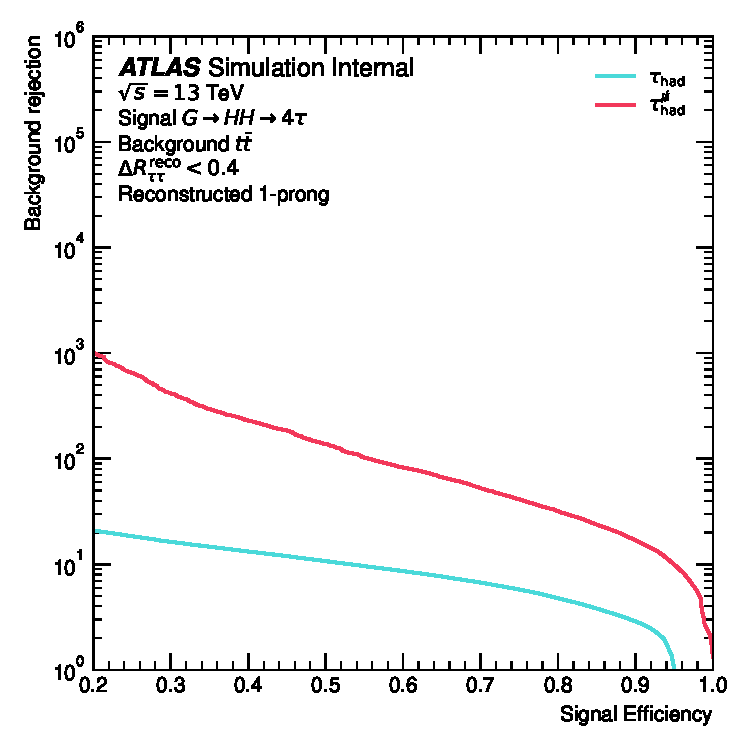
\includegraphics[width=0.5\textwidth]{plots_dev_fin/roc_1p.pdf}\label{fig:murm:roc_1p}}
                \subfloat[]{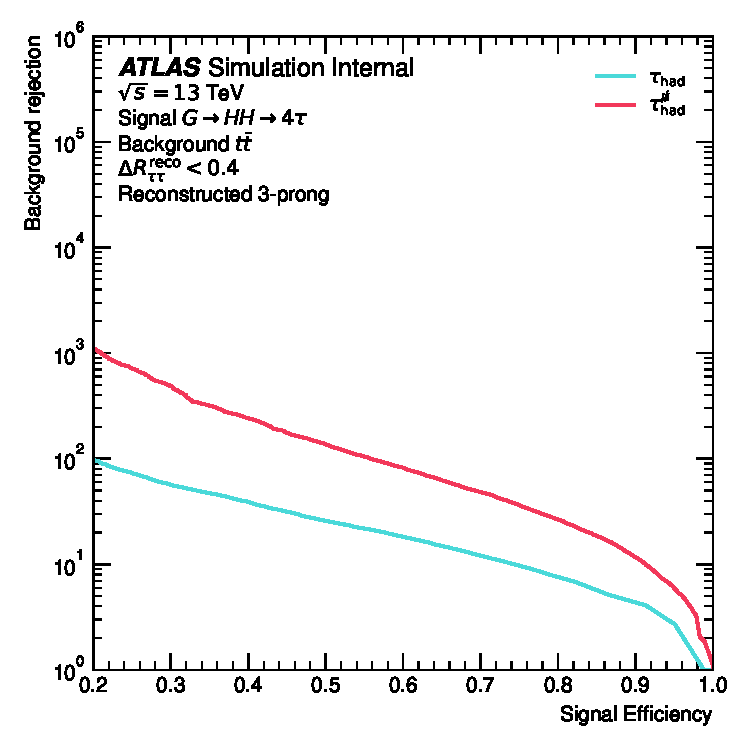
\includegraphics[width=0.5\textwidth]{plots_dev_fin/roc_3p.pdf}\label{fig:murm:roc_3p}}
                \caption{The receiver operating characteristic (ROC) curves with and without muon removal. 
                (\protect\subref{fig:murm:roc_1p}) shows the reconstructed 1-prong case, 
                (\protect\subref{fig:murm:roc_3p}) shows the 3-prong case.}
                \label{fig:murm:roc}
            \end{center}
        \end{figure}

        To demonstrate the performance of the $\tauhadmurm$ method in reconstructing and 
        identifying di-$\tau$ systems within the \GHHFourtau process, 
        Figure~\ref{fig:murm:effi_mass} presents the combined $\tauhad$ reconstruction and 
        identification efficiencies as a function of the truth-level Graviton mass. 
        The efficiencies shown correspond to the identification of individual di-$\tau$ systems originating from Higgs boson decays.
        Compared to the standard ATLAS TauID, the $\tauhadmurm$ method demonstrates a complete recovery 
        in the identification efficiency for both 1-prong and 3-prong $\tauhad$ decays for high-mass $\GHHFourtau$ samples.
        % This is a potential physics channel that future studies can exploit using the $\tauhadmurm$ method. 
        \begin{figure}[hbtp]
            \begin{center}
                \subfloat[]{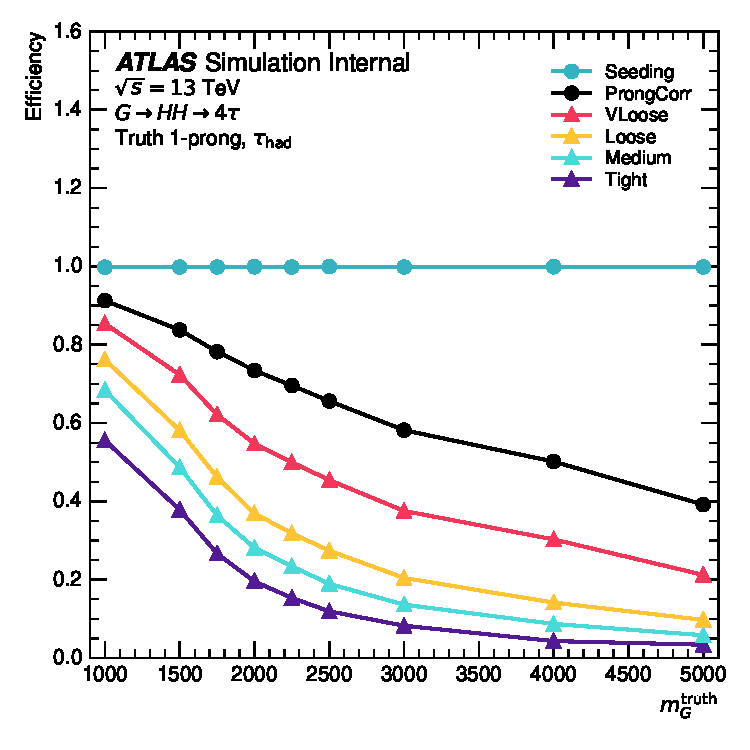
\includegraphics[width=0.50\textwidth]{plots_dev_fin/eff_nocut_mG_off_1p.pdf} \label{fig:murm:effi_mass_std_1p}}  
                \subfloat[]{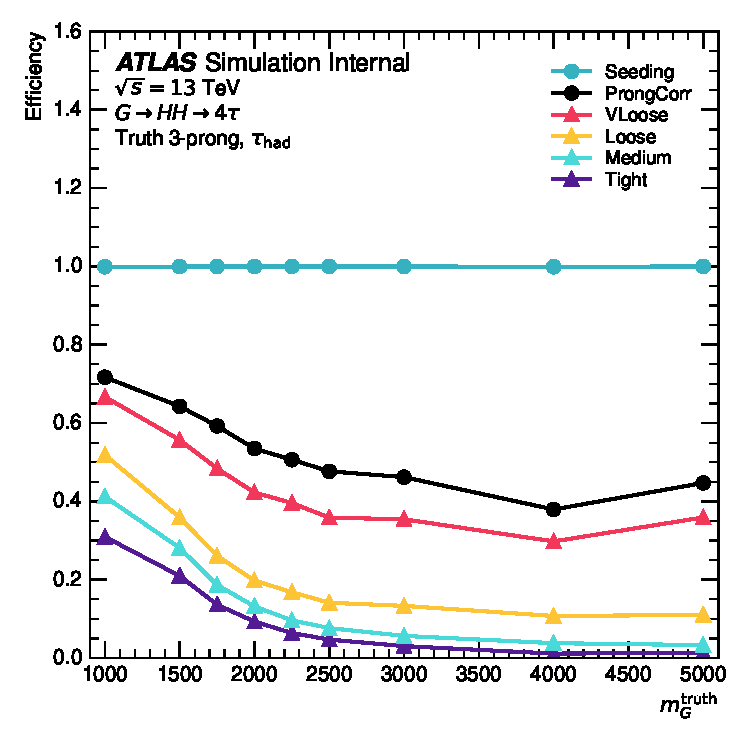
\includegraphics[width=0.50\textwidth]{plots_dev_fin/eff_nocut_mG_off_3p.pdf} \label{fig:murm:effi_mass_std_3p}}  
                \\
                \subfloat[]{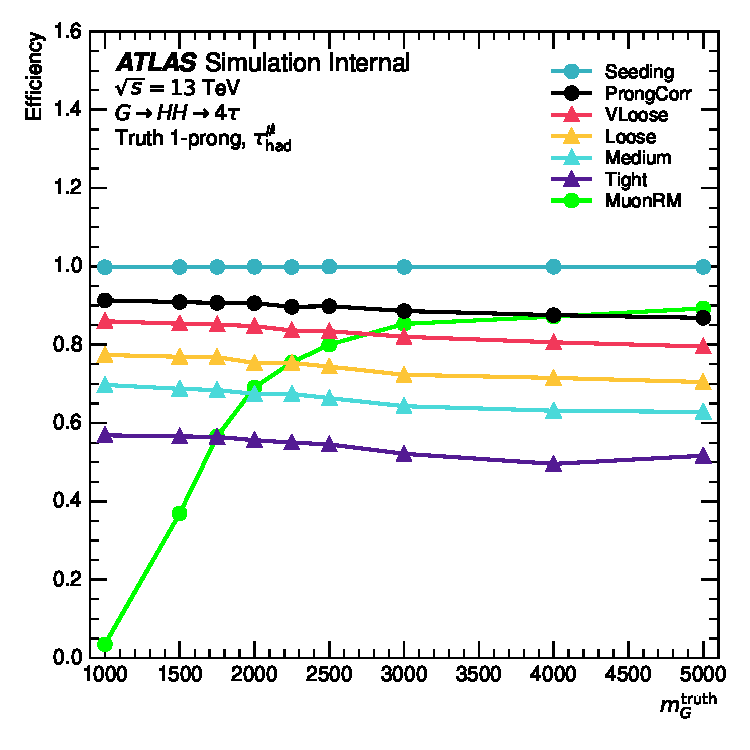
\includegraphics[width=0.50\textwidth]{plots_dev_fin/eff_nocut_mG_new_1p.pdf}\label{fig:murm:effi_mass_new_1p}}
                \subfloat[]{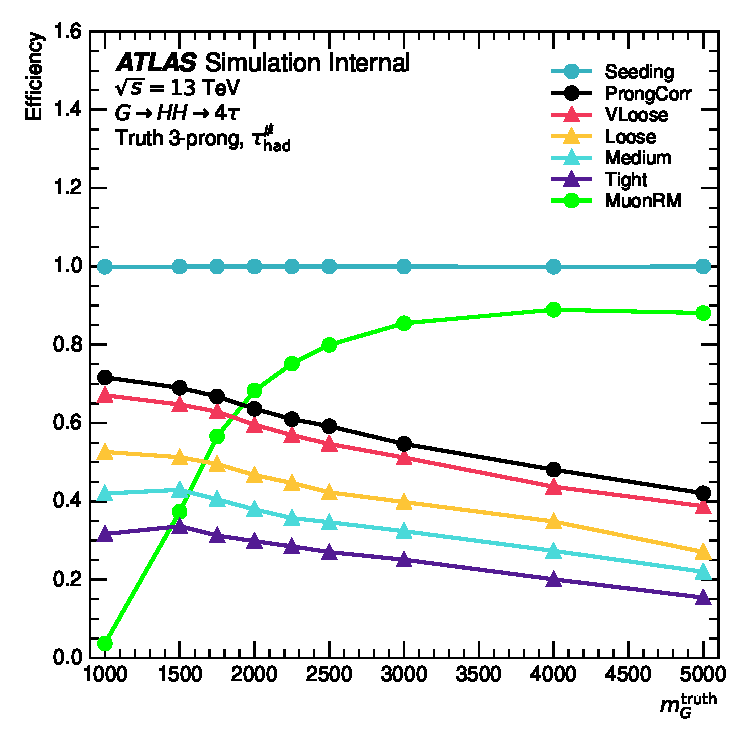
\includegraphics[width=0.50\textwidth]{plots_dev_fin/eff_nocut_mG_new_3p.pdf}\label{fig:murm:effi_mass_new_3p}}
                \caption{The signal efficiencies of the TauID working points, as a function of the truth-level Graviton mass, $m_G^\mathrm{truth}$, 
                    for truth 1-prong~(\protect\subref{fig:murm:effi_mass_std_1p}) and 3-prong~(\protect\subref{fig:murm:effi_mass_std_3p}) $\tauhad$ with the standard ATLAS TauID;
                    and for truth 1-prong~(\protect\subref{fig:murm:effi_mass_new_1p}) and 3-prong~(\protect\subref{fig:murm:effi_mass_new_3p}) $\tauhad$ with the $\tauhadmurm$ method.
                    The efficiencies shown correspond to the identification of individual di-$\tau$ systems originating from Higgs boson decays.
                    The ``Seeding'' lines indicate the efficiency 
                    of a truth-level $\tauhad$ being reconstructed as $\tauseed$. 
                    the ``ProngCorr'' line shows the efficiency of a truth-level $\tauhad$ being 
                    reconstructed with the correct number of associated charged-particle tracks.
                    The ``MuonRM'' lines show the efficiency of 
                    a muon being removed inside the $\tauseed$.
                }
                \label{fig:murm:effi_mass}
            \end{center}
        \end{figure}

\FloatBarrier

\section{Validation of the $\tauhadmurm$ method in the $\Zttmuhad$ channel} \label{sec:Zttbench}
    \subsection{The collinear assumptions and event reconstruction} \label{sec:collinear_assumptions_and_evt_reco}
        The $\tauhadmurm$ method was developed for searches like high-mass BSM physics, such as the \GHH process, 
        as described in Section~\ref{sec:murm}. However, it is useful to test its performance considering a SM process.
        The Drell-Yan production of a $Z$ boson in association with high-$p_T$ jets from QCD initial-state 
        radiation is considered as benchmark process.

        The detector signature of the boosted $\Zttmuhad$ process includes one hadronically decaying $\tau$ and a muon, 
        in association with significant missing transverse momentum ($\MET$) from the neutrinos produced in the two 
        $\tau$ decays. In this case, the hadronically decaying 
        $\tau$ and the muon are likely to fall within the same $\tauseed$ jet. In well measured events, the vector sum 
        of the transverse momenta of the three neutrinos dominates the measured $\MET$, which in azimuth direction should lie 
        between the observed muon and the $\tauhad$. Also, on average, the $\MET$ should be closer in azimuth to the muon, 
        because the leptonic decay produces two neutrinos and the hadronic decay only one.

        Without incorporating $\MET$, reconstructing the Z invariant mass is not possible. However, it is possible to approximate 
        the momenta of the neutrinos with the collinear assumptions~\cite{ELLIS1988221} as follows:
        \begin{itemize}
            \item the transverse momenta of the three neutrinos dominate the measured $\MET$, and other contributions are negligible;
            \item each $\tau$ lepton is sufficiently boosted such that the neutrino (or pair of neutrinos) produced in its decay is collinear with its visible decay products
            \footnote{In events in which the $\MET$ lies outside the azimuthal angle 
                between the visible decay products of the tau leptons (e.g., due to detector resolution), the 
                $\MET$ is projected onto the direction of the nearest visible decay, and the neutrino momentum 
                associated with the other tau lepton is set to zero. Furthermore, events for which collinear 
                reconstruction is not possible, i.e., with $\MET$ deviating by more than $90^{\circ}$ from the muon 
                or the $\tauhadmurm$ in $\deltaphi$, are discarded.}.
        \end{itemize}
        Together with the momenta of the visible decay products, this procedure allows the momenta of 
        the two tau leptons, and hence the momentum, transverse momentum ($\ptcol$), and mass ($\mcol$) 
        of the system produced by the decay of the $Z$ boson, to be reconstructed.
        The jets recoiling against the Z boson are reconstructed using the anti-$k_t$ algorithm with a radius 
        parameter of 0.4, which operates on topological clusters calibrated to the EM scale~\cite{JETM-2018-05}.
    \subsection{Event-selection} \label{sec:ZttSelection}
        Candidate events are required to be triggered by an un-prescaled single-muon trigger or an un-prescaled $\MET$ trigger.
        The thresholds of the $\pt$ required to fire each trigger vary for different data-taking periods. For the single muon trigger,
        the $\pt$ requirement for triggers with object isolation requirement ranges from 20-26~$\GeV$, while the $\pt$ threshold for non-isolated muons remains constant at 50~$\GeV$. 
        The \MET triggers have a $\pt$ threshold of 70~$\GeV$ for the 2015 data-taking period and remain constant at 110~$\GeV$ for the rest of Run~2. 
        Approximately 97\% of  $\Zttmuhad$ MC events that pass the final signal selection criteria pass the trigger selection.
        For the signal-region (SR) selection, events passing the trigger requirements are required 
        to have at least one muon-removal $\tauhad$ object with $\pt > 15~\GeV$ and a RNN TauID score > 0.1, 
        excluding pseudorapidity ranges $1.37 < |\eta| < 1.52$ and $|\eta| > 2.5$. This selection 
        implies that at least one reconstructed muon passing ``Medium'' ID is inside the cone of the selected 
        $\tauhadmurm$. An additional $\pt > 10~\GeV$ requirement on the corresponding muon is imposed. 
        In this study, the overlap removal (OLR) between muons and $\tauhad$ candidates is turned off. 
        The default overlap removal algorithm as described in Ref.~\cite{HIGG-2019-09} would remove 
        the $\tauhadmurm$ candidates if the muon removal method is successful. 
        To suppress background from events containing heavy flavour jets, events are vetoed if they 
        contain any jet that satisfies the DL1d based $b$-tagging algorithm at an 85\% efficiency working point~\cite{FTAG-2019-07}.
        The invariant mass, $\mvis$, of the visible $\tmth$ system is required to satisfy $\mvis > 5$~GeV. 
        The signed $\deltaphi$ between the muon and $\MET$ ($\deltamumet$) is required to be $-0.1 < \deltamumet < 0.4$ . 
        The sign of $\deltamumet$ is determined by the direction of the $\tauhad$. 
        If the $\MET$ is inside the opening angle of the muon and the $\tauhad$ or if the $\MET$ is outside 
        the opening angle but closer to the muon, then the sign is positive; otherwise, it is negative. 
        Since the focus of the analysis is the boosted $\Zttmuhad$ process, a loose requirement $\mcol > 40$~GeV, 
        and a requirement $\ptcol > 250$~GeV are applied. 
        To study the QCD multijets background contributions not described by the MC, 
        a control-region (CR) is defined with the same selection requirements as the SR, except that the
        muon and $\tauhadmurm$ have the same charge, and there is no requirement on $\deltamumet$ or 
        number of jets passing the $b$-tagging requirement.
        Table~\ref{tab:murm:evt_sel} summaries the event-selection requirements for SR and CR.
        \begin{table}[htbp]
            \caption{Summary of event-selection requirements}
            \label{tab:murm:evt_sel}
            \centering
            \scriptsize
            \begin{tabular}{lcc}
                \toprule
                Object & Signal-Region Selection & Control-Region Selection \\
                \midrule
                $\tauhadmurm$  & \begin{tabular}{c} $0 < |\eta| < 1.37$ or $1.52 < |\eta| < 2.5$ \\ Jet RNN score > 0.1 \\ $\pt > 15$~GeV \\ 1 or 3 charged tracks \end{tabular}   & \begin{tabular}{c} $0 < |\eta| < 1.37$ or $1.52 < |\eta| < 2.5$ \\ Jet RNN score > 0.1 \\ $\pt > 15$~GeV \\ 1 or 3 charged tracks \end{tabular} \\
                \midrule
                $\mu$          & \begin{tabular}{c} $\pt > 10~\GeV$ \\ ``Medium'' ID \end{tabular}                                      & \begin{tabular}{c} $\pt > 10~\GeV$ \\ ``Medium'' ID \end{tabular} \\       
                \midrule
                $\tmth$ system & \begin{tabular}{c} $\mvis > 5~\GeV$ \\ $-0.1 < \deltamumet < 0.4$ \\ $\mcol > 40~\GeV$ \\ $\ptcol > 250~\GeV$ \\ no $b$-tag jet at 85\% efficiency working point \\ Opposite Sign muon and $\tauhadmurm$ \end{tabular} &     \begin{tabular}{c} $\mvis > 5~\GeV$ \\ $\mcol > 40~\GeV$ \\ $\ptcol > 250~\GeV$ \\ Same Sign muon and $\tauhadmurm$\end{tabular} \\
                \bottomrule
            \end{tabular}
        \end{table}

        Figures~\ref{fig:murm:RNN_score}$-$\ref{fig:murm:pt_mu} illustrate the distributions of selected variables in the SR and CR. 
        As shown in Figure~\ref{fig:murm:m_col}, the data and MC predictions 
        agree well for $\mcol > 40$~GeV in both the SR and CR, indicating that QCD processes not modelled 
        by the MC simulations contribute negligibly to the background in the selected signal sample. The collinear 
        mass reconstruction effectively reconstructs the di-tau system mass, as seen in the peak corresponding to the $Z$ boson mass 
        in Figure~\ref{fig:murm:m_col}(a). The shape of the \mcol distribution for signal 
        Drell-Yan events is very different from that seen
        in inclusive production, with a much larger fraction of the signal events in the 
        region $40 < \mcol < 70$ GeV relative to that at the Z boson peak.  
        This is a result of the sharply falling distribution in Z boson \pT for Drell-Yan 
        production, coupled with the fact that the opening angle of boosted \tmth systems 
        decreases with decreasing \mcol.
        Due to the the $\mcol > 40$~GeV requirement, the number of events with $\ptcol$ below 250~GeV is very low. 
        This highlights the fact that the $\tauhadmurm$ reconstruction picks up $\tauhad$ only with a sufficiently high boost. 
        An excess of data compared to the MC prediction is observed in the $\pt < 35 \GeV$ region within the SR. 
        Further investigation has identified this discrepancy as a result of mis-modelling of the $\tauhad$ kinematics in 
        the $\Ztautau$ MC simulation~\cite{Dong:2899443}.
        % No significant excess of signal events around the Higgs boson mass is observed. This is consistent with expectations, 
        % given the lower production cross-section of the Higgs boson compared to the $Z$ boson.
        \begin{figure}[htbp]
            \centering
            \subfloat[]{
                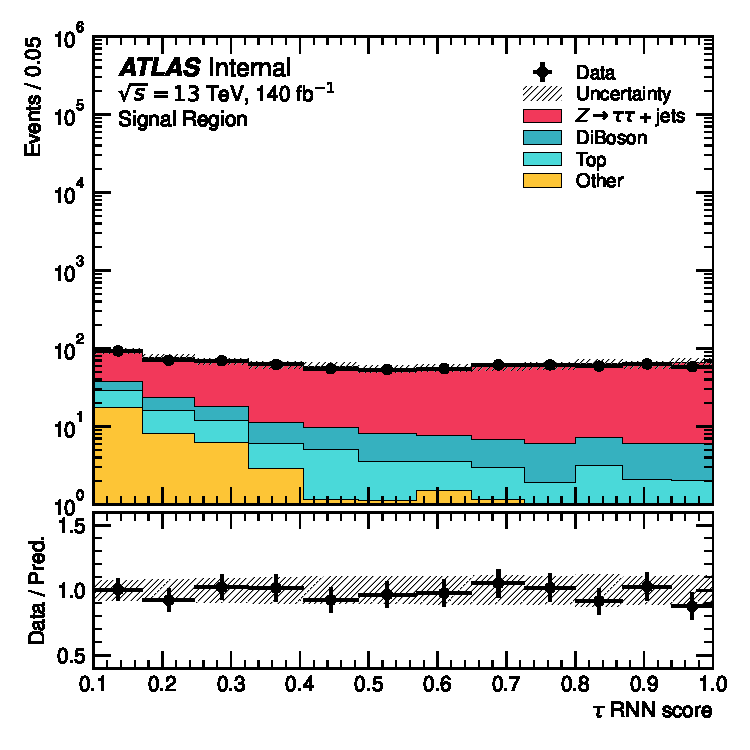
\includegraphics[width=0.50\textwidth]{plots_ztt_rebin_scaled_syst/leading_tau_rnn_SR.pdf}
                \label{fig:murm:SR_RNN_score}
            }
            \subfloat[]{
                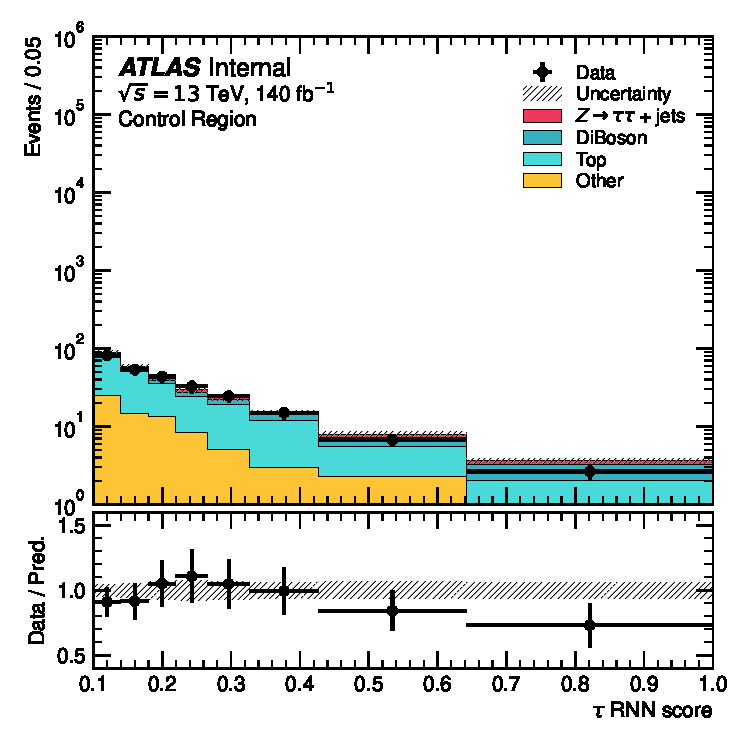
\includegraphics[width=0.50\textwidth]{plots_ztt_rebin_scaled_syst/leading_tau_rnn_CR_new_final.pdf}
                \label{fig:murm:CR_RNN_score}
            }
            \caption{
                The distribution of the RNN jet score for $\tauhadmurm$: (\protect\subref{fig:murm:SR_RNN_score}) in the SR and,
                (\protect\subref{fig:murm:CR_RNN_score}) in the CR. 
                ``Top'' represents the predicted contributions from the SM $\ttbar$, single-top, and $tW$ processes. 
                ``DiBoson'' indicates the contributions from $WW$, $WZ$, and $ZZ$ processes. 
                ``Other'' includes the contributions from the $Z\rightarrow ll$+jets and $W$+jets background processes. 
                ``$\Ztautau$+jets'' represents the contributions from the signal process.
                The uncertainties shown include both statistical and systematic uncertainties.
            }
            \label{fig:murm:RNN_score}
        \end{figure}

        \begin{figure}[htbp]
            \centering
            \subfloat[]{
                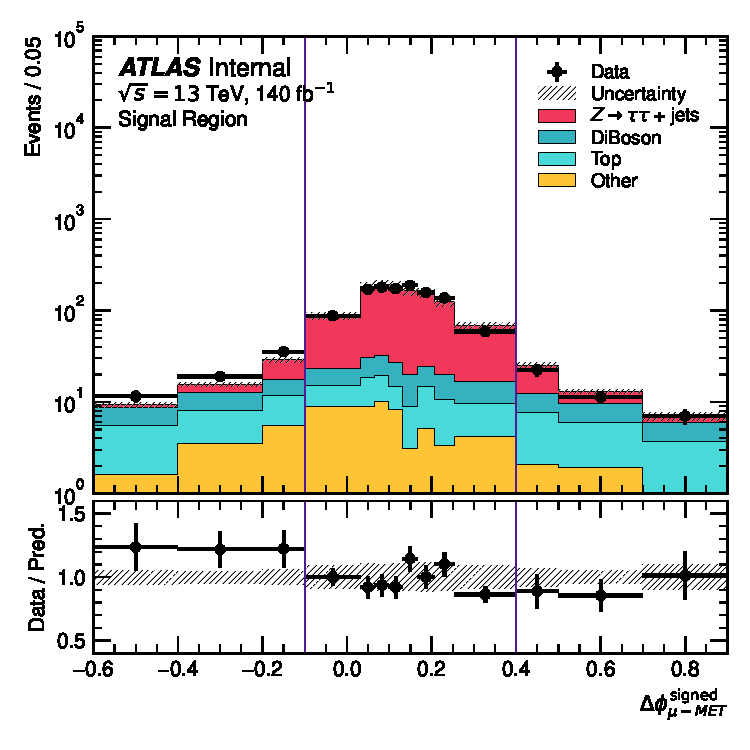
\includegraphics[width=0.50\textwidth]{plots_ztt_rebin_scaled_syst/omega_noscale_SR.pdf}
                \label{fig:murm:SR_s_dphi}
            }
            \subfloat[]{
                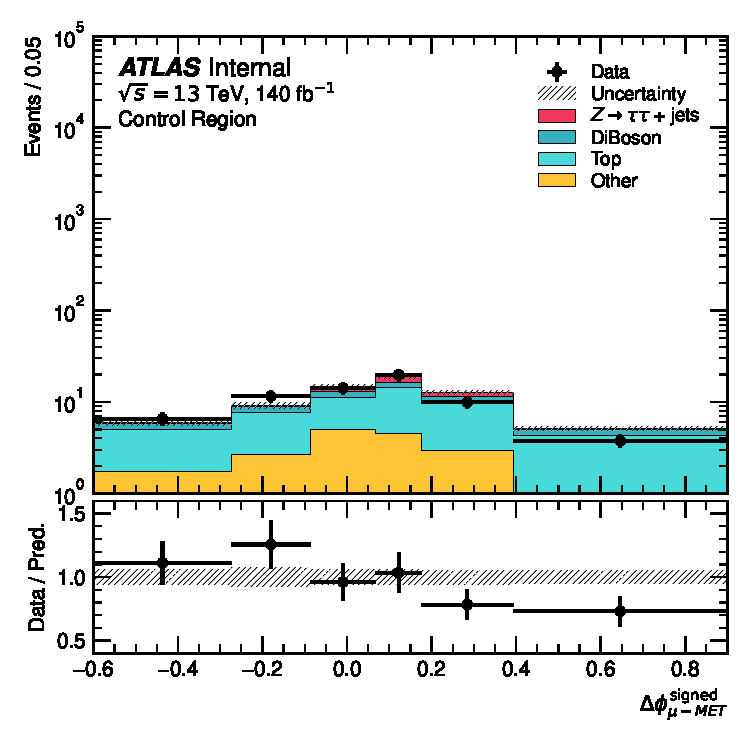
\includegraphics[width=0.50\textwidth]{plots_ztt_rebin_scaled_syst/omega_noscale_CR_new_final.pdf}
                \label{fig:murm:CR_s_dphi}
            }
            \caption{
                The distribution of $\deltamumet$ with all other event-selection criteria 
                applied in the SR is shown in (\protect\subref{fig:murm:SR_s_dphi}); 
                the straight lines indicate the positions of the selection requirements.
                The same distribution in the CR is shown in (\protect\subref{fig:murm:CR_s_dphi}). 
                ``Top'' represents the predicted contributions from the SM $\ttbar$, single-top, and $tW$ processes. 
                ``DiBoson'' indicates the contributions from $WW$, $WZ$, and $ZZ$ processes. 
                ``Other'' includes the contributions from the $Z\rightarrow ll$+jets and $W$+jets background processes. 
                ``$\Ztautau$+jets'' represents the contributions from the signal process.
                The uncertainties shown include both statistical and systematic uncertainties.
            }
            \label{fig:murm:s_dphi}
        \end{figure}

        \begin{figure}[htbp]
            \centering
            \subfloat[]{
                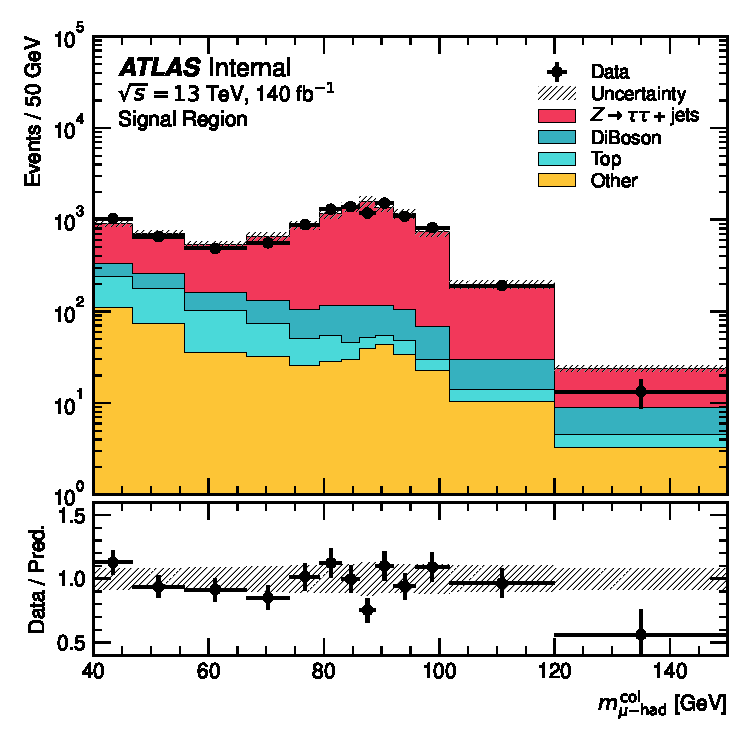
\includegraphics[width=0.50\textwidth]{plots_ztt_rebin_scaled_syst/m_tt_colin_SR.pdf}
                \label{fig:murm:SR_m_col}
            }
            \subfloat[]{
                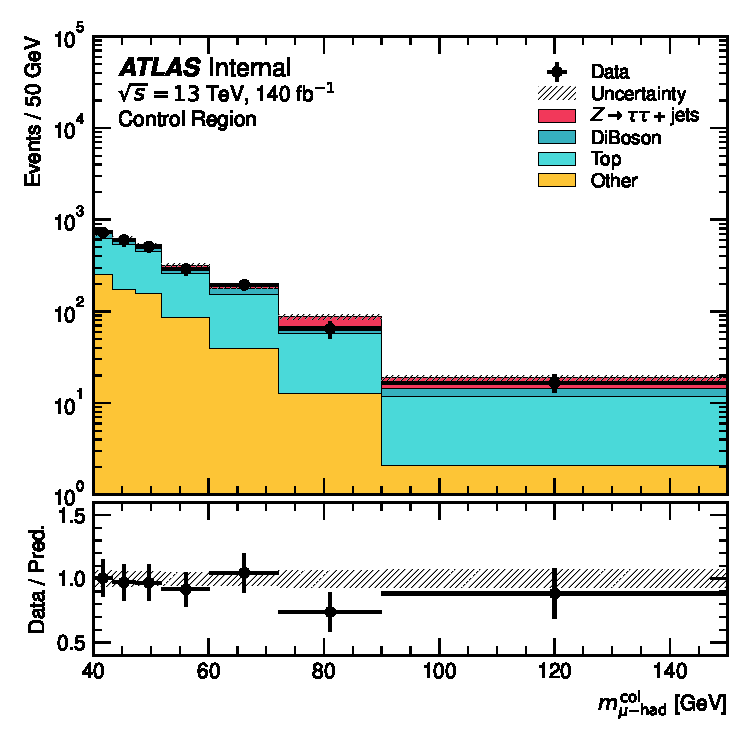
\includegraphics[width=0.50\textwidth]{plots_ztt_rebin_scaled_syst/m_tt_colin_CR_new_final.pdf}
                \label{fig:murm:CR_m_col}
            }
            \caption{
                The distribution of the $\mcol$: (\protect\subref{fig:murm:SR_m_col}) in the SR, and,
                (\protect\subref{fig:murm:CR_m_col}) in the CR. 
                ``Top'' represents the predicted contributions from the SM $\ttbar$, single-top, and $tW$ processes. 
                ``DiBoson'' indicates the contributions from $WW$, $WZ$, and $ZZ$ processes. 
                ``Other'' includes the contributions from the $Z\rightarrow ll$+jets and $W$+jets background processes. 
                ``$\Ztautau$+jets'' represents the contributions from the signal process.
                The uncertainties shown include both statistical and systematic uncertainties.
            }
            \label{fig:murm:m_col}
        \end{figure}

        \begin{figure}[htbp]
            \centering
            \subfloat[]{
                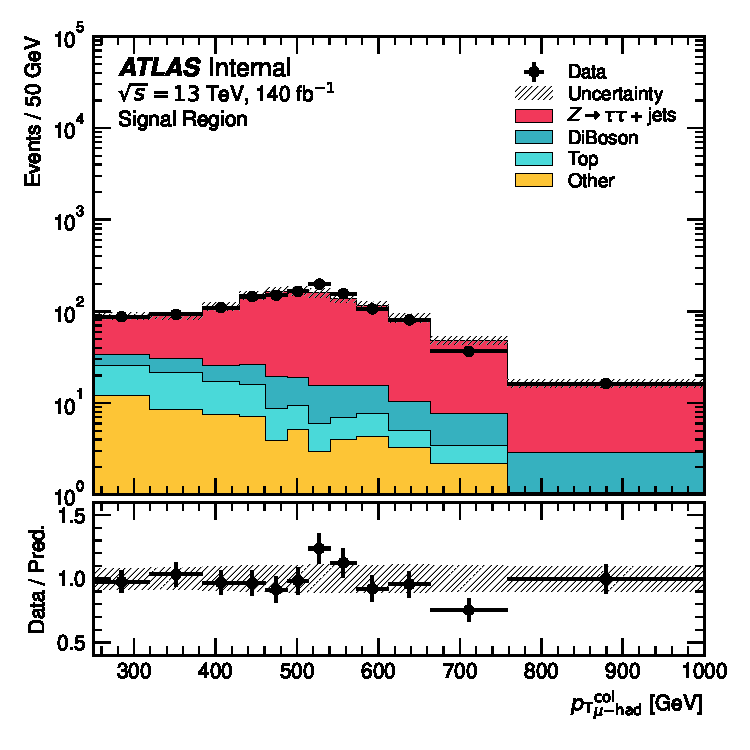
\includegraphics[width=0.50\textwidth]{plots_ztt_rebin_scaled_syst/pt_tt_colin_SR.pdf}
                \label{fig:murm:SR_pt_col}
            }
            \subfloat[]{
                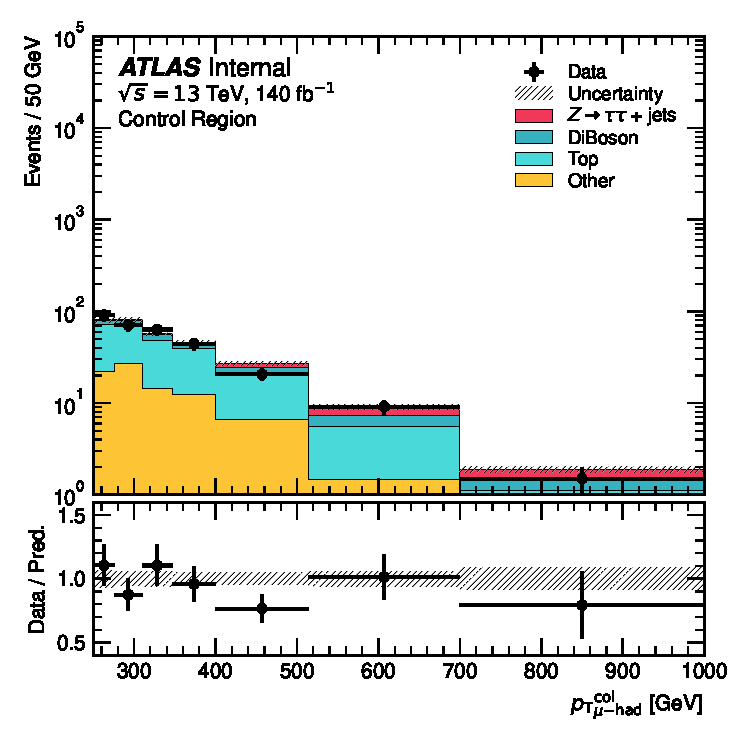
\includegraphics[width=0.50\textwidth]{plots_ztt_rebin_scaled_syst/pt_tt_colin_CR_new_final.pdf}
                \label{fig:murm:CR_pt_col}
            }
            \caption{
                The distribution of the $\ptcol$: (\protect\subref{fig:murm:SR_pt_col}) in the SR, and,
                (\protect\subref{fig:murm:CR_pt_col}) in the CR. 
                ``Top'' represents the predicted contributions from the SM $\ttbar$, single-top, and $tW$ processes. 
                ``DiBoson'' indicates the contributions from $WW$, $WZ$, and $ZZ$ processes. 
                ``Other'' includes the contributions from the $Z\rightarrow ll$+jets and $W$+jets background processes. 
                ``$\Ztautau$+jets'' represents the contributions from the signal process.
                The uncertainties shown include both statistical and systematic uncertainties.
            }
            \label{fig:murm:pt_col}
        \end{figure}

        \begin{figure}[htbp]
            \centering
            \subfloat[]{
                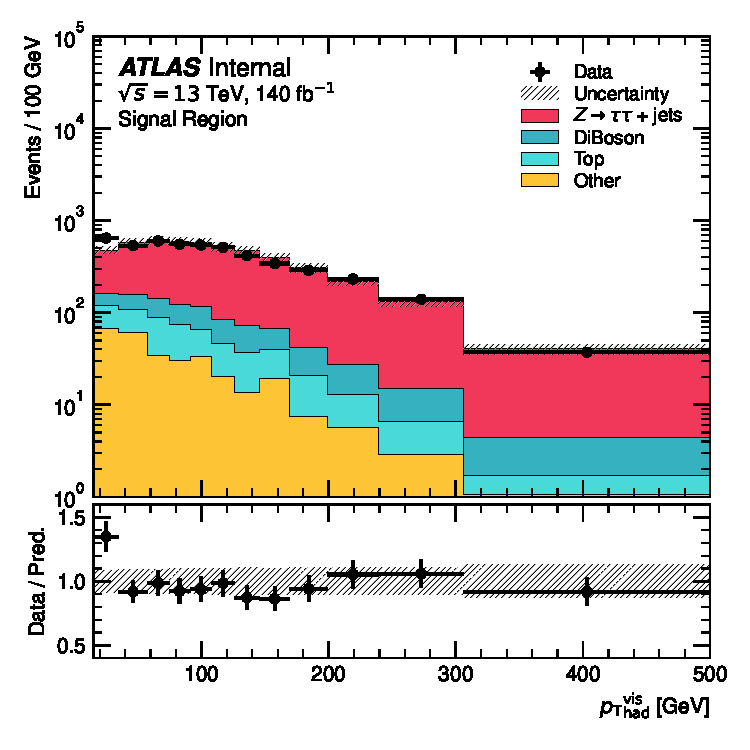
\includegraphics[width=0.50\textwidth]{plots_ztt_rebin_scaled_syst/leading_tau_pt_SR.pdf}
                \label{fig:murm:SR_pt_tau}
            }
            \subfloat[]{
                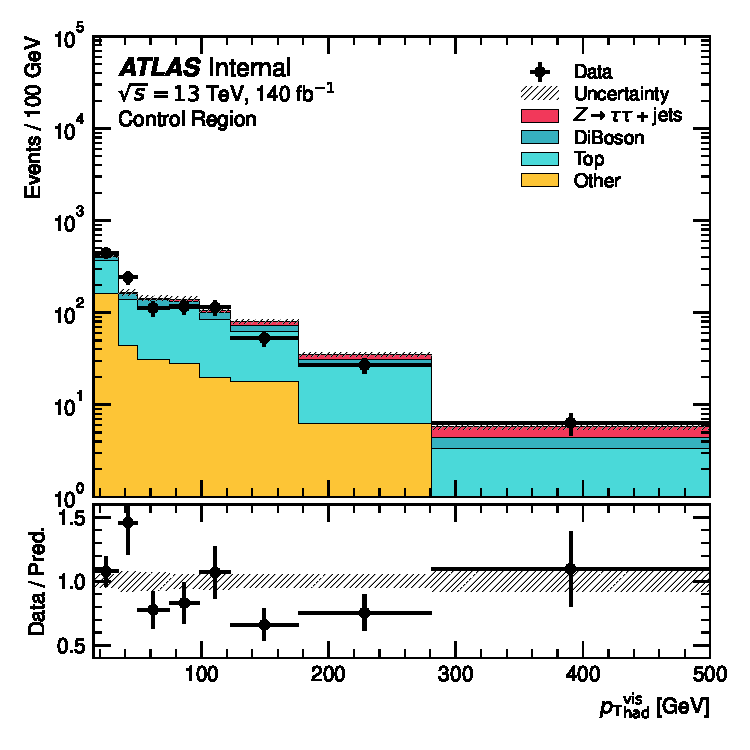
\includegraphics[width=0.50\textwidth]{plots_ztt_rebin_scaled_syst/leading_tau_pt_CR_new_final.pdf}
                \label{fig:murm:CR_pt_tau}
            }
            \caption{
                The distribution of the \pt of the $\tauhadmurm$: (\protect\subref{fig:murm:SR_pt_tau}) in the SR  and,
                (\protect\subref{fig:murm:CR_pt_tau}) in the CR. 
                ``Top'' represents the predicted contributions from the SM $\ttbar$, single-top, and $tW$ processes. 
                ``DiBoson'' indicates the contributions from $WW$, $WZ$, and $ZZ$ processes. 
                ``Other'' includes the contributions from the $Z\rightarrow ll$+jets and $W$+jets background processes. 
                ``$\Ztautau$+jets'' represents the contributions from the signal process.
                The uncertainties shown include both statistical and systematic uncertainties.
            }
            \label{fig:murm:pt_tau}
        \end{figure}

        \begin{figure}[htbp]
            \centering
            \subfloat[]{
                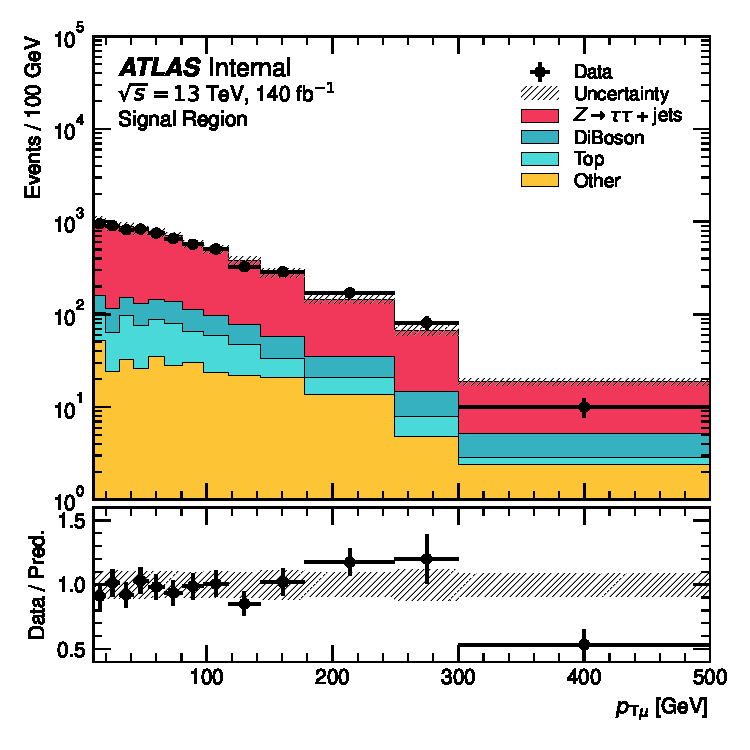
\includegraphics[width=0.50\textwidth]{plots_ztt_rebin_scaled_syst/muon_pt_SR.pdf}
                \label{fig:murm:SR_pt_mu}
            }
            \subfloat[]{
                \includegraphics[width=0.50\textwidth]{plots_ztt_rebin_scaled_syst/muon_pt_CR_new_final.pdf}
                \label{fig:murm:CR_pt_mu}
            }
            \caption{
                The distribution of the \pt of the muon removed from the $\tauhadmurm$: 
                (\protect\subref{fig:murm:SR_pt_mu}) in the SR and,
                (\protect\subref{fig:murm:CR_pt_mu}) in the CR. 
                ``Top'' represents the predicted contributions from the SM $\ttbar$, single-top, and $tW$ processes. 
                ``DiBoson'' indicates the contributions from $WW$, $WZ$, and $ZZ$ processes. 
                ``Other'' includes the contributions from the $Z\rightarrow ll$+jets and $W$+jets background processes. 
                ``$\Ztautau$+jets'' represents the contributions from the signal process.
                The uncertainties shown include both statistical and systematic uncertainties.
            }
            \label{fig:murm:pt_mu}
        \end{figure}

    \subsection{Systematic uncertainties} \label{sec:sys_uncertainties}
        The dominant source of systematic uncertainty in the comparison between the observed and expected yields in the SR is the modelling of the cross-section 
        for $Z$ boson production. As discussed in Section~\ref{sec:DataAndMCs}, a +10\% 
        correction is applied to the predicted numbers for $\Ztautau$ events, 
        with the full size of this correction quoted as a systematic uncertainty.

        The most significant sources of experimental systematic uncertainties are TauID and tau energy scale~(4\%), 
        jet energy scale and resolution~(2\%), \MET~(2\%)~\cite{Baron:2887993}, and luminosity~(0.8\%)~\cite{DAPR-2021-01}.
\section{Results} \label{sec:results}
    % In this section, the results of the $\Ztautau$ benchmark analysis are presented, 
    % focusing on the signal and background distributions, event yields in the signal and control 
    % regions, and some important observations. 
    In order to understand the performance improvement 
    comparing to the standard ATLAS $\tauhad$ reconstruction and identification,
    Figure~\ref{fig:murm:SRcmp} shows comparisons between the data and MC predictions for \mcol\ distributions corresponding to various signal selections;
    Figure~\ref{fig:murm:SR_m} shows the SR defined in Section~\ref{sec:ZttSelection};
    Figure~\ref{fig:murm:SR_std_m} shows the sample \SRstd, which uses the standard ATLAS $\tauhad$ candidates;
    without the muon removal, but otherwise corresponds to the same event-selection as SR;
    Figure~\ref{fig:murm:SR_tight_m} shows the sample \SRtight, which
    imposes an additional ``tight'' RNN TauID requirement on the $\tauhadmurm$ candidates, but otherwise corresponds
    to the SR selection;
    Figure~\ref{fig:murm:SR_tight_std_m} shows the sample \SRtightstd, which
    imposes an additional ``tight'' RNN TauID requirement and uses the standard $\tauhad$, without muon removal.
    
    \begin{figure}[htbp]
        \centering
        \subfloat[]{
            \includegraphics[width=0.50\textwidth]{plots_ztt_rebin_scaled_syst/m_tt_colin_SR_cmp.pdf}
            \label{fig:murm:SR_m}
        }
        \subfloat[]{
            \includegraphics[width=0.50\textwidth]{plots_ztt_rebin_scaled_syst/m_tt_colin_SR_std_cmp.pdf}
            \label{fig:murm:SR_std_m}
        }
        \\
        \subfloat[]{
            \includegraphics[width=0.50\textwidth]{plots_ztt_rebin_scaled_syst/m_tt_colin_SR_tight_cmp.pdf}
            \label{fig:murm:SR_tight_m}
        }
        \subfloat[]{
            \includegraphics[width=0.50\textwidth]{plots_ztt_rebin_scaled_syst/m_tt_colin_SR_tight_std_cmp.pdf}
            \label{fig:murm:SR_tight_std_m}
        }
        \caption{The distributions of $\mcol$ corresponding to the various signal selections defined in the text: 
            (\protect\subref{fig:murm:SR_m}) SR, 
            (\protect\subref{fig:murm:SR_std_m}) \SRstd, 
            (\protect\subref{fig:murm:SR_tight_m}) \SRtight, and
            (\protect\subref{fig:murm:SR_tight_std_m})  \SRtightstd.
            SR, $\SRtight$ and CR are with the $\tauhadmurm$ method, while $\SRstd$ and $\SRtightstd$ are with the standard ATLAS TauID.
        }
        \label{fig:murm:SRcmp}
    \end{figure}
    Table~\ref{tab:murm:n_evt} shows the event yields corresponding to the various signal selections defined previously,
    and the CR. The number of events observed in 
    the ATLAS Run 2 data are given, as well as the SM-predicted contributions from signal and background processes. 
        
    Compared with the  the standard ATLAS TauID, the $\tauhadmurm$ achieves around 
    three times more signal events in the SR, while maintaining a similar number of background events. 
    In the \SRtight\ region, the number of signal events 
    is four times higher than using the nominal $\tauhadstd$, again while maintaining a similar number of background events.
    \begin{table}[htbp]
        \caption{
            Event yields in different event-selections, as defined in the text. 
            SR, $\SRtight$ and CR are with the $\tauhadmurm$ method, while $\SRstd$ and $\SRtightstd$ are with the standard ATLAS TauID.
            The uncertainties quoted are statistical only. The $Z\rightarrow\tau\tau$ contribution
            is scaled by +10\% to account for the difference between the MC prediction and the data.
        }
        \label{tab:murm:n_evt}
        \centering
        \scriptsize
        \begin{tabular}{l|cc|cc|c}
            \toprule
                                    & SR                & $\SRstd$                  & $\SRtight$                & $\SRtightstd$                         & CR   \\
            \midrule
            Data                    & $1155 \pm 34$     & $616 \pm 25$              & $705 \pm 27$              & $210 \pm 14$                          & $286 \pm 17$     \\ 
            MC total                & $1188 \pm 10$     & $574 \pm 8$               & $733 \pm 7$               & $223 \pm 4$                           & $302 \pm 7$ \\
            \midrule
            $\Ztautau$              & $958\pm 8$        & $339 \pm 4$               & $646 \pm 6$               & $124 \pm 2$                           & $20 \pm 1$ \\
            Di-boson                & $93 \pm 1$        & $37 \pm 1$                & $51 \pm 1$                & $15 \pm 0$                            & $39 \pm 1$ \\
            Top                     & $70 \pm 3$        & $153 \pm 5$               & $26 \pm 2$                & $67 \pm 3$                            & $165 \pm 5$  \\
            Other                   & $66 \pm 4$        & $45 \pm 4$                & $10\pm 2$                 & $17 \pm 2$                            & $78 \pm 4$ \\
            \bottomrule
        \end{tabular}
    \end{table}
    Subtracting the expected background yield in the SR of $230\pm 5$ events gives a 
    measured yield for $\Zttmuhad$ of $925 \pm 34$ events. 
    This can be compared to the expected yield for \Zttmuhad\ of $958 \pm 8~\text{(stat.)}\pm~115~\text{(syst.)}$ events. 
    Adding all sources of statistical and systematic uncertainty results in a total uncertainty of 12\%. 
    The ratio between the background-subtracted data and the expected signal yields is $0.97 \pm 0.12$. 


\FloatBarrier

\section{Summary and conclusion} \label{sec:conclusion}
    In this chapter, the case of a highly boosted pair of $\tau$ leptons is considered, 
    in which one $\tau$ decays produce a muon and the other $\tau$ decays hadronically, 
    with the visible decay products reconstructed within a single $\tauseed$ jet. In such 
    cases, the standard ATLAS TauID for hadronically decaying $\tau$ leptons fails due 
    to the presence of the nearby muon.

    The development of a muon-removal procedure using samples of high-mass $\GHHFourtau$ 
    events is described. This $\tauhadmurm$ method recovers the \tauhad\ reconstruction and identification 
    efficiencies to the level expected for isolated \tauhad\ decays for all TauID working 
    points. The measurement precision for the kinematic properties of the visible \tauhad\ 
    system is similarly recovered. The $\tauhadmurm$ objects are benchmarked by selecting 
    a sample of highly boosted $\Zttmuhad$ final states using the complete Run 2 dataset 
    recorded by the ATLAS detector. Good agreement is found between data and MC predictions 
    in both the signal $\Zttmuhad$ region and in a control-region in which the muon and 
    \tauhad\ candidate have same-sign charges. The comparison of rates in the signal 
    region gives a ratio between the background-subtracted data and the expected 
    signal yields of $0.97 \pm 0.12$. 

    The results presented in this chapter demonstrate the effectiveness of the $\tauhadmurm$ 
    objects in enhancing the signal sensitivity of the boosted $\tmth$ channel. The 
    observed good agreement between the data and the SM theory predictions in the signal 
    region reaffirms the robustness of the newly developed object. 
